\documentclass[12pt,a4paper]{report}

\usepackage[utf8]{inputenc}
\usepackage[T1]{fontenc}
\usepackage{mathptmx} % Times Roman font matching the reference CUSAT report
\usepackage[a4paper,left=1.0in,right=1.0in,top=1.0in,bottom=1.0in]{geometry}
\usepackage{setspace}
\usepackage{graphicx}
\usepackage{amsmath,amssymb}
\usepackage{booktabs}
\usepackage{array}
\usepackage{longtable}
\usepackage{xcolor}
\usepackage{listings}
\usepackage{enumitem}
\usepackage{caption}
\usepackage[hidelinks]{hyperref}

\onehalfspacing
\setlength{\parindent}{1.5em}
\setlength{\parskip}{0.4em}
\emergencystretch=1.5em

% Page border toggle for front-matter pages (Pages 2--Contents, matching CUSAT format)
\newif\iffrontborder
\frontborderfalse
\AddToHook{shipout/background}{%
    \iffrontborder
        \put(31pt,-811pt){\framebox(533pt,780pt){}}%
    \fi
}

% Centered uppercase CONTENTS, LIST OF FIGURES, LIST OF TABLES titles
\renewcommand{\contentsname}{\centering \Large \textbf{CONTENTS}}
\renewcommand{\listfigurename}{\centering \Large \textbf{LIST OF FIGURES}}
\renewcommand{\listtablename}{\centering \Large \textbf{LIST OF TABLES}}

% Code listing style matching reference report (cream background, line numbers, syntax colors)
\definecolor{codebg}{HTML}{F7F7F0}
\definecolor{codekw}{HTML}{007020}
\definecolor{codestr}{HTML}{BA2121}
\definecolor{codecmt}{HTML}{408080}
\definecolor{codenum}{HTML}{888888}

\lstdefinestyle{pythonstyle}{
    language=Python,
    backgroundcolor=\color{codebg},
    basicstyle=\ttfamily\footnotesize\linespread{1.05}\selectfont,
    keywordstyle=\color{codekw}\bfseries,
    stringstyle=\color{codestr},
    commentstyle=\color{codecmt}\itshape,
    numbers=left,
    numberstyle=\tiny\color{codenum},
    numbersep=8pt,
    frame=none,
    breaklines=true,
    breakatwhitespace=true,
    showstringspaces=false,
    tabsize=4,
    xleftmargin=12pt,
    framexleftmargin=8pt,
    aboveskip=10pt,
    belowskip=10pt
}
\lstset{style=pythonstyle}

\begin{document}

% ==============================================================================
% PAGE 1: OUTER COVER PAGE (Unnumbered, No Border, With CUSAT Logo)
% ==============================================================================
\newcommand{\printtitlecontent}{%
\begin{center}
    \vspace*{0.8cm}
    {\Large \textbf{MINI PROJECT REPORT}}\\[0.35cm]
    {\large \textbf{SAR-GUIDED SATELLITE CLOUD REMOVAL}}\\[0.15cm]
    {\normalsize \textbf{(ADVERSARIALLY SHARPENED ECRFORMER ARCHITECTURE)}}\\[0.9cm]

    {\normalsize \textit{Submitted in partial fulfillment of the requirements for the award of}}\\[0.35cm]
    {\normalsize \textit{the degree of}}\\[0.7cm]

    {\Large \textbf{\textit{M.Sc. Computer Science with Specialization in}}}\\[0.25cm]
    {\Large \textbf{\textit{Artificial Intelligence}}}\\[0.6cm]

    {\normalsize \textit{2025--2027}}\\[0.7cm]

    {\normalsize By}\\[0.45cm]

    {\large \textbf{AGNAL K V (25020460)}}\\[0.2cm]
    {\large \textbf{BIVIN BALU (25020320)}}\\[0.2cm]
    {\large \textbf{VAISHNAV T PRAKASH (25020382)}}\\[0.75cm]

    {\large \textbf{DEPARTMENT OF COMPUTER APPLICATIONS}}\\[0.45cm]

    
\includegraphics[width=3.5cm]{backend/assets/cusat_logo.png}\\[0.5cm]

    {\Large \textbf{COCHIN UNIVERSITY OF SCIENCE}}\\[0.2cm]
    {\Large \textbf{AND TECHNOLOGY}}\\[0.35cm]
    {\large \textbf{NOVEMBER 2026}}
\end{center}
}

\begin{titlepage}
\thispagestyle{empty}
\frontborderfalse
\printtitlecontent
\end{titlepage}

% ==============================================================================
% PAGE 2: INNER COVER PAGE (Unnumbered, With Page Border & CUSAT Logo)
% ==============================================================================
\newpage
\thispagestyle{empty}
\frontbordertrue
\printtitlecontent
\newpage

% ==============================================================================
% PAGE 3: CERTIFICATE (Unnumbered, With Page Border & CUSAT Logo)
% ==============================================================================
\thispagestyle{empty}
\begin{center}
    \vspace*{0.6cm}
    {\large \textbf{DEPARTMENT OF COMPUTER APPLICATIONS}}\\[0.25cm]
    {\large \textbf{COCHIN UNIVERSITY OF SCIENCE AND TECHNOLOGY}}\\[0.55cm]
    
\includegraphics[width=3.5cm]{backend/assets/cusat_logo.png}\\[0.75cm]
    {\Large \textbf{CERTIFICATE}}\\[0.9cm]
\end{center}

\noindent This is to certify that the mini project report on the topic \textbf{``SAR-GUIDED SATELLITE CLOUD REMOVAL (ADVERSARIALLY SHARPENED ECRFORMER ARCHITECTURE)''} submitted in partial fulfillment of the requirements for the award of the Degree of M.Sc. Computer Science with a Specialization in Artificial Intelligence is a record of bona fide work done by \textbf{AGNAL K V (25020460)}, \textbf{BIVIN BALU (25020320)}, and \textbf{VAISHNAV T PRAKASH (25020382)} during the period of their study in the Department of Computer Applications at Cochin University of Science and Technology.

\vfill

\noindent{\fontsize{11}{14.5}\selectfont
\begin{tabular}[t]{@{}l@{}}
    \textbf{Signature of Supervisor}\\[0.35cm]
    \mbox{\textbf{Dr.~Sabu~M~K}}\\
    Professor\\
    Department of Computer Applications\\
    Cochin University of Science and Technology
\end{tabular}%
\hfill
\begin{tabular}[t]{@{}r@{}}
    \textbf{Signature of Head of Department}\\[0.35cm]
    \mbox{\textbf{Dr.~Vinod~P}}\\
    Professor \& Head\\
    Department of Computer Applications\\
    Cochin University of Science and Technology
\end{tabular}}
\vspace*{0.8cm}

\newpage

% ==============================================================================
% PAGE 4: DECLARATION (Unnumbered, With Page Border)
% ==============================================================================
\thispagestyle{empty}
\begin{center}
    \vspace*{1.2cm}
    {\Large \textbf{DECLARATION}}\\[1.2cm]
\end{center}

\noindent We hereby declare that the mini project report on the topic \textbf{``SAR-GUIDED SATELLITE CLOUD REMOVAL (ADVERSARIALLY SHARPENED ECRFORMER ARCHITECTURE)''} submitted in partial fulfillment of the requirements for the award of the Degree of M.Sc. Computer Science with a Specialization in Artificial Intelligence is a record of bona fide work done by us during our course M.Sc. Computer Science with specialization in Artificial Intelligence, under the supervision and guidance of \mbox{\textbf{Dr.~Sabu~M~K}} in the Department of Computer Applications, Cochin University of Science and Technology.

\vfill

\noindent
\begin{tabular}{@{}p{0.46\textwidth}p{0.50\textwidth}@{}}
    Place: & \textbf{Signature} \\[0.35cm]
    & \textbf{AGNAL K V (25020460)} \\[0.25cm]
    & \textbf{BIVIN BALU (25020320)} \\[0.25cm]
    & \textbf{VAISHNAV T PRAKASH (25020382)} \\
\end{tabular}
\vspace*{1.0cm}

\newpage

% ==============================================================================
% PAGE 5: ACKNOWLEDGEMENT (Unnumbered, With Page Border)
% ==============================================================================
\thispagestyle{empty}
\begin{center}
    \vspace*{1.0cm}
    {\Large \textbf{ACKNOWLEDGEMENT}}\\[1.1cm]
\end{center}

\noindent We thank God for granting us the strength, wisdom, and perseverance to be able to finish this mini project report.

\vspace{0.35cm}
\noindent We hereby acknowledge our sincere thanks to all those who inspired and supported us during the preparation of this mini project report. We express our deepest gratitude to \mbox{\textbf{Dr.~Vinod~P}}, Head of the Department and Professor, for his constant inspiration and for maintaining an enriching academic atmosphere.

\vspace{0.35cm}
\noindent We take this opportunity to express our profound gratitude to our project supervisor, \mbox{\textbf{Dr.~Sabu~M~K}}, Professor, Department of Computer Applications, for his scholarly guidance, invaluable suggestions, and continuous encouragement throughout the course of this work.

\vspace{0.35cm}
\noindent We thank our friends and fellow classmates for their support and valuable comments, and our families for their unrelenting faith in us, which inspired us throughout the ordeal.

\vspace{0.35cm}
\noindent This mini project report is the fruit of all their encouragement and support, and we hope it turns out to be our genuine effort and learning in this endeavor.

\vfill

\noindent
\begin{tabular}{@{}p{0.46\textwidth}p{0.50\textwidth}@{}}
    Place: & Signature: \\[0.35cm]
    Date: & \textbf{AGNAL K V (25020460)} \\[0.25cm]
    & \textbf{BIVIN BALU (25020320)} \\[0.25cm]
    & \textbf{VAISHNAV T PRAKASH (25020382)} \\
\end{tabular}
\vspace*{0.8cm}

\newpage

% ==============================================================================
% PAGE 6+: CONTENTS, LIST OF FIGURES, LIST OF TABLES (Unnumbered, With Page Border)
% ==============================================================================
\pagestyle{empty}
\addtocontents{toc}{\protect\thispagestyle{empty}}
\addtocontents{lof}{\protect\thispagestyle{empty}}
\addtocontents{lot}{\protect\thispagestyle{empty}}
{\singlespacing
\tableofcontents
\newpage
\listoffigures
\newpage
\listoftables
\newpage
}

% ==============================================================================
% ABSTRACT (Page 1, Numbering Starts Here, No Page Border)
% ==============================================================================
\frontborderfalse
\pagestyle{plain}
\setcounter{page}{1}
\pagenumbering{arabic}
\phantomsection
\addcontentsline{toc}{chapter}{Abstract}
\thispagestyle{plain}
\begin{center}
    \vspace*{0.4cm}
    {\LARGE \textbf{Abstract}}\\[1.0cm]
\end{center}

\noindent Optical Earth observation satellites such as the European Space Agency's Sentinel-2 provide high-resolution multispectral imagery ($10\text{ m/pixel}$) essential for agricultural crop monitoring, flood mapping, deforestation tracking, and urban planning. However, passive optical sensors rely on reflected sunlight and are severely obstructed by cloud cover, which obscures more than $50\%$ of the Earth's land surface at any given moment. This project, \textbf{SAR-Guided Satellite Cloud Removal}, addresses this fundamental remote sensing bottleneck by architecting and training a multimodal deep learning pipeline that fuses cloud-penetrating active C-band Synthetic Aperture Radar (SAR) backscatter from Sentinel-1 ($\text{VV}$ and $\text{VH}$ polarisations) with corrupted 4-band Sentinel-2 optical imagery ($\text{B04}$ Red, $\text{B03}$ Green, $\text{B02}$ Blue, and $\text{B08}$ Near-Infrared) on the co-registered \textbf{SEN12MS-CR (\texttt{ROIs1970\_fall})} benchmark dataset ($33{,}468$ training patches and $1{,}115$ validation patches).

The core restoration engine is built upon an $8.31$-million-parameter adapted hybrid Convolutional--Transformer generator (\textbf{\texttt{ECRformerAdaptedModel}}) featuring a two-branch decoupled modality stem, zero-information-loss \texttt{PixelUnshuffle}/\texttt{PixelShuffle} spatial sampling, Convolutional Block Attention Modules (\texttt{CBAM 1ca2+1sa2}), and a Restormer-style Multi-Dconv Head Transposed Attention (\textbf{MDTA}) bottleneck. Because MDTA computes attention across feature channels ($[C\times C] = [256\times 256]$) rather than spatial pixels ($[HW\times HW]$), the generator is trained efficiently on $128\times 128$ crops while executing inference directly on full $256\times 256$ scenes ($0.04\text{ seconds/scene}$). A critical engineering milestone during the project lifecycle was overcoming the severe over-smoothing (``blurry gray smudge'') produced by standard pixel-wise $L_1 + \text{SSIM}$ training ($13.3\%$ detail retention) due to conditional-mean averaging and $1$--$2\text{ pixel}$ SAR-to-optical orbital co-registration shifts. By introducing \textbf{Opaque Cloud Cutout} ($\text{prob}=0.65$) to prevent thin-cloud optical shortcuts, \textbf{Scale-Decoupled $L_1$ Loss} ($4\times 4$ and $8\times 8$ pooled colour supervision inside clouds), \textbf{Cloud-Boosted Structural Losses} (VGG-16 perceptual, multi-scale signed gradients, edge correlation, and $16\times 16$ local contrast matching), and an \textbf{11-channel High-Pass Spectral-Normalized PatchGAN critic}, the finalized pipeline boosts in-cloud texture sharpness by $+47.6\%$ to $+133.3\%$ ($\text{Detail Ratio} \approx 0.90$--$0.93$) while maintaining $30.07$--$31.93\text{ dB}$ in-cloud PSNR and $100\%$ radiometric fidelity on cloud-free terrain via a soft-mask blending gate.

\newpage

% ==============================================================================
% CHAPTER 1: INTRODUCTION
% ==============================================================================
\chapter{Introduction}

\section{Overview}
Satellite remote sensing forms the backbone of modern environmental intelligence, climate monitoring, disaster response, and precision agriculture. Passive multispectral satellites, most notably the European Space Agency's (ESA) Sentinel-2 constellation, capture rich surface reflectance across visible and near-infrared wavelengths at a spatial resolution of $10\text{ meters per pixel}$. However, because optical instruments operate at nanometric wavelengths ($\lambda \approx 490$--$842\text{ nm}$) that are smaller than typical atmospheric water droplets ($\approx 10\,\mu\text{m}$), non-selective Mie scattering causes thick clouds to act as an impenetrable white barrier. Globally, more than half of the Earth's land surface is occluded by cloud cover at any instant, rendering a massive fraction of optical satellite acquisitions unusable.

Conversely, Sentinel-1 carries an active C-band Synthetic Aperture Radar (SAR) transceiver operating at a microwave wavelength of approximately $5.5\text{ cm}$ ($5.5\times 10^7\text{ nm}$). Because this wavelength is roughly $5{,}500$ times larger than cloud water droplets, microwave pulses pass through thick cloud layers, rain, and atmospheric haze with virtually zero attenuation, operating day and night. While SAR imagery captures detailed surface geometry, road networks, building footprints, and vegetation volume, it lacks natural spectral colour and suffers from coherent speckle noise. The \textbf{SAR-Guided Satellite Cloud Removal} project bridges this physical divide by combining the structural penetrative power of Sentinel-1 SAR with the spectral richness of Sentinel-2 optical imagery using an adversarially sharpened hybrid Transformer architecture (\textbf{ECRformer}).

\section{Problem Statement}
Optical Earth observation satellites such as Sentinel-2 are indispensable for agricultural monitoring, flood mapping, deforestation tracking, and disaster management, yet passive optical sensors rely on reflected sunlight and cannot see through clouds. With more than $50\%$ of the Earth's land surface covered by clouds at any given moment, a vast proportion of acquired satellite imagery is rendered unusable due to opaque white cloud cover and atmospheric haze.

Conventional cloud removal techniques suffer from critical limitations in real-world remote sensing scenarios:
\begin{enumerate}
    \item \textbf{Failure of Optical-Only Inpainting Under Thick Clouds:} Spatial interpolation methods attempt to fill cloudy regions using surrounding clear-sky pixels, which fails completely when thick clouds obscure $50\%$--$95\%$ of a satellite scene and leave no local optical reference.
    \item \textbf{Temporal Lag in Multi-Temporal Compositing:} Stitching together cloud-free pixels from satellite passes taken weeks apart fails during time-critical events such as flash floods, wildfire progression, or seasonal crop harvesting where the ground changes rapidly.
    \item \textbf{Loss of Ground Texture and Clear-Sky Fidelity in Standard Deep Models:} Existing deep learning cloud removal networks trained with standard pixel-wise losses tend to produce blurry, over-smoothed reconstructions inside thick clouds and inadvertently distort pixels in regions that were already cloud-free.
\end{enumerate}
Therefore, there is a pressing need for a robust, single-date cloud removal mechanism capable of penetrating thick cloud cover to reconstruct sharp, spectrally accurate ground imagery without altering unoccluded terrain.

\section{Objectives}
The primary objective of this project is to design, train, and deploy an automated \textbf{SAR-Guided Satellite Cloud Removal} system using an adapted hybrid Transformer architecture (\textbf{ECRformer}). Specifically, the project aims to:
\begin{itemize}
    \item \textbf{Develop a Multimodal Cloud Removal Mechanism:} Fuse cloud-penetrating Sentinel-1 Synthetic Aperture Radar (SAR: $\text{VV}, \text{VH}$) with cloudy 4-band Sentinel-2 optical imagery ($\text{B04}$ Red, $\text{B03}$ Green, $\text{B02}$ Blue, and $\text{B08}$ NIR) to reconstruct missing ground information underneath thick clouds.
    \item \textbf{Ensure True Radar-Guided Structural Recovery:} Train the $8.31\text{M}$-parameter \texttt{ECRformerAdaptedModel} generator so that roads, rivers, building footprints, and agricultural boundaries hidden beneath opaque clouds are accurately recovered from SAR radar geometry.
    \item \textbf{Achieve High-Frequency Texture Sharpness:} Eliminate the blurry ``smudge'' effect inside reconstructed cloud regions through a composite perceptual and High-Pass PatchGAN adversarial training pipeline.
    \item \textbf{Preserve $100\%$ Clear-Sky Radiometric Integrity:} Integrate a soft cloud-probability mask blending gate ($\hat{Y} = (1-M)\odot S2_{\text{cloudy}} + M\odot P_{\text{dir}}$) so that cloud-free pixels remain $100\%$ identical to the original satellite observation.
    \item \textbf{Provide an Interactive Visual Evaluation Platform:} Build a lightweight React + FastAPI web application with a split-screen comparison slider for inspecting cloudy inputs, SAR radar maps, and restored cloud-free outputs across diverse terrains.
\end{itemize}

\section{Scope of the Project}
The scope of this project encompasses the complete end-to-end satellite restoration workflow on the \texttt{SEN12MS-CR} (\texttt{ROIs1970\_fall}) dataset: raw floating-point \texttt{.npz} tensor ingestion, ESA \texttt{s2cloudless} probability mask refinement, physical decibel normalization, $128\times 128$ joint adversarial training, $256\times 256$ full-scene quantitative benchmarking across four cloud-cover strata ($0$--$25\%$, $25$--$50\%$, $50$--$75\%$, and $75$--$100\%$), public model weight distribution on Hugging Face, and a lightweight browser-based visual comparison application. The system is designed for $10\text{ m/pixel}$ co-registered Sentinel-1/Sentinel-2 patches and focuses on single-date cloud removal rather than multi-temporal time-series compositing.

\section{Organization of the Report}
The remainder of this report is organized as follows: Chapter 2 reviews the scientific literature on optical cloud removal, SAR-optical fusion, channel-transposed Vision Transformers, and adversarial sharpening. Chapter 3 presents the System Analysis, comparing existing baseline approaches against our proposed architecture and evaluating technical, operational, and economic feasibility. Chapter 4 details the \texttt{ECRformerAdaptedModel} architecture and the \texttt{SEN12MS-CR} dataset structure. Chapter 5 specifies the hardware and software requirements. Chapter 6 formulates the complete mathematical foundations, including worked numerical derivations for radar normalization, MDTA channel attention, Scale-Decoupled $L_1$, and High-Pass PatchGAN filtering. Chapter 7 documents the PyTorch implementation and the critical engineering pivot from the blurry Pre-GAN baseline to the 7-loss adversarial recipe. Chapter 8 presents multi-stage visual and quantitative evaluation results. Finally, Chapter 9 concludes the report and outlines future research directions.

% ==============================================================================
% CHAPTER 2: LITERATURE REVIEW
% ==============================================================================
\chapter{Literature Review}

\section{Evolution of Optical Cloud Removal in Remote Sensing}
Early approaches to cloud removal in optical satellite imagery relied on spatial interpolation (inpainting) or multi-temporal compositing. Spatial inpainting methods copy textures from cloud-free borders into the cloud interior; while effective for narrow clouds or sensor scan-line gaps, they fail catastrophically when clouds cover $60\%$--$95\%$ of a $256\times 256$ scene because no surrounding context exists. Multi-temporal methods stitch together cloud-free pixels acquired over multiple weeks, but rapid surface changes---such as flash floods, crop harvesting, or wildfire progression---render time-delayed composites obsolete for urgent monitoring.

\section{Physics of Active SAR vs. Passive Optical Multimodal Fusion}
To overcome the physical limits of optical-only restoration, Meraner et al. (2020) introduced the landmark \textbf{SEN12MS-CR} dataset and the \texttt{DSen2-CR} residual convolutional network, establishing the paradigm of SAR-guided optical cloud removal. Sentinel-1 C-band SAR ($\lambda \approx 5.5\text{ cm}$) provides two complementary physical channels:
\begin{itemize}
    \item \textbf{VV Polarisation (Vertical Transmit, Vertical Receive):} Highly sensitive to surface dielectric constant, water boundaries, road networks, and urban corner reflectors ($\text{VV} \in [-25, 0]\text{ dB}$).
    \item \textbf{VH Polarisation (Vertical Transmit, Horizontal Receive):} Captures depolarised volume scattering inside three-dimensional tree canopies and agricultural crops ($\text{VH} \in [-35, 0]\text{ dB}$).
\end{itemize}
By conditioning a deep network on co-registered Sentinel-1 SAR, the underlying terrain geometry remains visible even under $100\%$ opaque cloud cover.

\section{Vision Transformers and Channel-Transposed Attention}
While Convolutional Neural Networks (CNNs) such as \texttt{DSen2-CR} excel at local edge extraction, their limited receptive fields struggle to propagate colour palette cues from distant clear-sky margins into large cloud cores. Vision Transformers (Vaswani et al., 2017) capture global context via self-attention, but standard spatial self-attention computes an $[HW\times HW]$ pixel-to-pixel affinity matrix whose memory complexity grows quadratically ($\mathcal{O}((HW)^2)$) and whose learned spatial dimensions break when changing resolution from training crops to full test scenes.

Zamir et al. (2022) resolved this bottleneck in \textbf{Restormer} by introducing \textbf{Multi-Dconv Head Transposed Attention (MDTA)}, which transposes the query and key projection axes to compute cross-covariance across feature channels ($[C\times C]$) rather than spatial pixels. Building upon this insight and pairing it with Convolutional Block Attention Modules (\textbf{CBAM}; Woo et al., 2018), the \textbf{ECRformer} architecture combines local depthwise separable convolutions with global channel-transposed attention at a fraction of standard Transformer compute cost.

\section{Adversarial Sharpening and the Perception--Distortion Trade-Off}
A pervasive failure mode across published SAR-optical cloud removal models (including \texttt{DSen2-CR} and standard $L_1$-trained Transformers) is severe texture smoothing inside thick clouds. Blau and Michaeli (2018) proved mathematically that distortion metrics (such as PSNR and MSE/$L_1$) and perceptual sharpness are fundamentally at odds when reconstructing uncertain high-frequency textures: the minimum-distortion estimator is the conditional expectation (a blurry average). Isola et al. (2017) demonstrated in \textbf{Pix2Pix} that a Markovian \textbf{PatchGAN} discriminator---stabilized via Spectral Normalization (Miyato et al., 2018) and Perceptual Feature Losses (Johnson et al., 2016)---forces generators to commit to crisp, realistic high-frequency textures rather than safe averages.

% ==============================================================================
% CHAPTER 3: SYSTEM ANALYSIS
% ==============================================================================
\chapter{System Analysis}

\section{Analysis of the Existing System}
Conventional satellite cloud removal pipelines typically feed concatenated SAR and cloudy optical tensors into a single convolutional stem and train the network end-to-end using pixel-wise $L_1$ or $\text{CHARBONNIER} + \text{SSIM}$ loss.

\subsection{Drawbacks of the Existing System}
\begin{enumerate}
    \item \textbf{Single-Stem Modality Interference:} Concatenating raw microwave SAR speckle directly with sunlight reflectance in the very first $3\times 3$ convolution forces shared filters to process incompatible physical distributions, degrading early feature extraction.
    \item \textbf{Vulnerability to the Thin-Cloud Optical Shortcut:} Because many training patches contain semi-transparent haze where ground edges leak through, standard models learn to copy and contrast-stretch the optical input while ignoring the SAR channels.
    \item \textbf{The 1--2 Pixel Radar Shift ``Double-Edge Penalty'':} Because Sentinel-1 (side-looking radar) and Sentinel-2 (nadir optical camera) are acquired from different orbital geometries, terrain relief causes subtle $1$--$2\text{ pixel}$ co-registration offsets. Under strict $1\times 1$ pixel $L_1$ loss, drawing a crisp road guided by SAR that is shifted by $1\text{ pixel}$ incurs double error compared to predicting a wide blurry smear.
    \item \textbf{Clear-Sky Radiometric Degradation:} Models that output a full neural reconstruction without soft-mask gating slightly alter the reflectance and blur fine details even in $100\%$ cloud-free regions of the image.
\end{enumerate}

\section{Proposed System Architecture}
Our proposed system introduces a \textbf{Dual-Phase Multimodal Pipeline} centered on an $8.31\text{M}$-parameter \texttt{ECRformerAdaptedModel} generator trained at $128\times 128$ crop scale with seven targeted loss functions and evaluated at native $256\times 256$ resolution with soft-mask radiometric preservation.

\subsection{Merits of the Proposed System}
\begin{itemize}
    \item \textbf{True SAR Structural Reliance via Opaque Cutout (Role M1):} By blinding $65\%$ of training clouds with a featureless $29\times 29$ average-pooled veil, our generator cannot cheat from faint optical leaks and genuinely learns to translate VV/VH radar echoes into roads, rivers, and field boundaries.
    \item \textbf{Shift-Tolerant Colour + Crisp Edge Decoupling (Roles M3 \& M4):} Our \textbf{Scale-Decoupled $L_1$ Loss} relaxes strict $1\times 1$ pixel $L_1$ by $80\%$ inside clouds and supervises regional colour on $4\times 4$ and $8\times 8$ pooled grids---eliminating the double-edge penalty---while VGG-16 and multi-scale gradient losses enforce sharp boundaries.
    \item \textbf{High-Pass PatchGAN Critic (Role M5):} An 11-channel Spectral-Normalized PatchGAN critic inspects both the predicted reflectance and its $5\times 5$ high-pass residual $R_{\text{HP}} = 10(x - \text{AvgPool}_{5\times 5}(x))$, penalizing blurry cloud regions $4\times$ more strictly than clear sky.
    \item \textbf{Train Small ($128^2$), Test Big ($256^2$):} Thanks to zero-loss \texttt{PixelUnshuffle} folding and $[256\times 256]$ MDTA channel attention, the network trains rapidly on a single GPU and scales seamlessly to full $256\times 256$ scenes at test time ($0.04\text{ s/patch}$).
\end{itemize}

\section{Feasibility Study}
A rigorous feasibility study was conducted across three operational dimensions prior to full-scale training.

\subsection{Technical Feasibility}
Training a hybrid Transformer generator alongside a frozen VGG-16 feature extractor and a 4-stage PatchGAN discriminator requires careful VRAM management. By utilizing $128\times 128$ random spatial crops during Phase 1 training, mixed-precision \texttt{Bfloat16}/\texttt{FP16} execution, and an Exponential Moving Average (\texttt{EMA}, decay $0.999$) shadow generator, the entire training loop fits comfortably within $8$--$12\text{ GB}$ of GPU VRAM on a single desktop workstation. At test time, VGG-16 and PatchGAN are discarded entirely, allowing full $256\times 256$ inference in just $40\text{ milliseconds}$.

\subsection{Operational Feasibility}
To ensure seamless usability for remote sensing analysts and academic evaluators, the project includes a standalone React + Vite web showcase featuring an interactive split-screen comparison slider (\texttt{CompareSlider.jsx}). Pre-exported multi-stage outputs allow instant browser-based inspection on any laptop without requiring local GPU drivers, while a FastAPI backend supports live \texttt{.npz} inference when a GPU or CPU PyTorch environment is active.

\subsection{Economic Feasibility}
The project relies entirely on open-access satellite missions (ESA Copernicus Sentinel-1 and Sentinel-2), the public \texttt{SEN12MS-CR} benchmark, and open-source software (PyTorch, FastAPI, React, Hugging Face Hub). Consequently, there are zero proprietary licensing fees or commercial cloud API costs.

% ==============================================================================
% CHAPTER 4: THE BASE MODEL AND DATASET
% ==============================================================================
\chapter{The Base Model and Dataset}

\section{The ECRformerAdaptedModel Architecture (8.31M Parameters)}
The core generator $G_{\theta}$ implemented in \texttt{backend/models/ecrformer\_model.py} is an hourglass encoder--decoder network containing exactly \textbf{8,316,228 trainable parameters} (\texttt{features\_start = 32}, \texttt{num\_blocks = [2, 2, 1, 1]}, \texttt{bottle\_neck = "tsa"}, \texttt{cbam = "1ca2+1sa2"}).

\subsection{Architectural Innovations}
\begin{itemize}
    \item \textbf{Decoupled Two-Branch Modality Stem:} Instead of feeding all 7 input channels into one convolution, Branch 0 applies $\text{Conv}_{7\times 7}(2 \to 16) + \text{BN} + \text{ReLU}$ exclusively to the 2 SAR channels ($\text{VV}, \text{VH}$), while Branch 1 applies $\text{Conv}_{7\times 7}(5 \to 16) + \text{BN} + \text{ReLU}$ to the 4 cloudy optical bands concatenated with the soft cloud mask $M$ (Role M2). The two 16-channel feature maps are then concatenated into a 32-channel fused representation.
    \item \textbf{Zero-Loss \texttt{PixelUnshuffle} and \texttt{PixelShuffle} Sampling:} Rather than discarding $75\%$ of spatial activations via strided pooling, each encoder stage downsamples by folding $2\times 2$ spatial neighborhoods into $4\times$ channels ($[B, C, 2H, 2W] \to [B, 4C, H, W]$) followed by a $3\times 3$ channel-compressing convolution ($32 \to 64 \to 128 \to 256$). The decoder mirrors this with \texttt{PixelShuffle} unfolding and three multi-scale skip-connection fusion bridges.
    \item \textbf{Hybrid Depthwise Conv + CBAM (\texttt{1ca2+1sa2}):} Each encoder/decoder stage executes residual depthwise-separable \texttt{ECRformerBlock} layers paired with Channel Attention (weighing spectral/radar channels) and Spatial Attention ($7\times 7$ conv highlighting cloud transition boundaries).
    \item \textbf{Mean-Prior Output Bias Initialization:} The final $3\times 3$ output head (\texttt{final\_conv}: $64 \to 4$) is initialized with bias values equal to the empirical clear-sky reflectance means of the dataset ($[0.0847,\; 0.0919,\; 0.1127,\; 0.1884]$ for Red, Green, Blue, and NIR), preventing early gradient shock against bright white clouds ($\approx 0.80$).
\end{itemize}

\section{The SEN12MS-CR (\texttt{ROIs1970\_fall}) Multimodal Dataset}
We train and evaluate our system on the \textbf{SEN12MS-CR} benchmark dataset (\texttt{ROIs1970\_fall} seasonal subset), utilizing a strict, non-overlapping split of \textbf{33,468 training patches} and \textbf{1,115 validation patches}, while holding out tile \texttt{s2\_139} as an untouched test region.

\subsection{Dataset Structure and Spectral/Radar Band Pedagogy}
Each sample is stored as a compressed 32-bit floating-point NumPy archive (\texttt{.npz}) covering a $256\times 256$ pixel grid at $10\text{ m/pixel}$ ground sampling distance ($2.56\text{ km}\times 2.56\text{ km}$). Unlike 8-bit JPEG images that clip values to $0$--$255$ across only 3 RGB channels, \texttt{.npz} tensors preserve scientific radiometric precision across all 6 physical sensor bands plus the cloud mask, as detailed in Table \ref{tab:dataset_structure}.

\begin{table}[htbp]
\centering
\caption{Structure of a Cached \texttt{SEN12MS-CR} (\texttt{ROIs1970\_fall}) \texttt{.npz} Patch}
\label{tab:dataset_structure}
\renewcommand{\arraystretch}{1.35}
\begin{tabular}{|p{2.3cm}|p{2.6cm}|p{9.2cm}|}
\hline
\textbf{Tensor Key} & \textbf{Shape \& Type} & \textbf{Physical Band Description \& Value Range} \\
\hline
\texttt{s2\_cloudy} & $[4, 256, 256]$ \texttt{float32} & Corrupted Sentinel-2 optical input in $[0.0, 1.0]$ (raw DN / $10{,}000$). Channels: \textbf{B04} (Red, $665\text{ nm}$), \textbf{B03} (Green, $560\text{ nm}$), \textbf{B02} (Blue, $490\text{ nm}$), and \textbf{B08} (Near-Infrared, $842\text{ nm}$). \\
\hline
\texttt{s1} & $[2, 256, 256]$ \texttt{float32} & Co-registered Sentinel-1 C-band SAR backscatter in decibels ($\text{dB}$), normalized to $[0.0, 1.0]$. Channel 0: \textbf{VV} $\in [-25, 0]\text{ dB}$ (surface roughness/buildings); Channel 1: \textbf{VH} $\in [-35, 0]\text{ dB}$ (3D vegetation volume scattering). \\
\hline
\texttt{s2\_clear} & $[4, 256, 256]$ \texttt{float32} & Co-registered cloud-free Sentinel-2 target reference $Y \in [0.0, 1.0]$ across bands $[\text{B04}, \text{B03}, \text{B02}, \text{B08}]$. \\
\hline
\texttt{mask} & $[1, 256, 256]$ \texttt{float32} & Soft cloud probability mask $M \in [0.0, 1.0]$ generated via ESA \texttt{s2cloudless} and refined via 3-step morphological filtering ($0 = \text{clear sky}$, $1 = \text{opaque cloud}$). \\
\hline
\texttt{cf} & Scalar \texttt{float32} & Scene-level cloud fraction $\in [0.0, 1.0]$ used to stratify validation benchmarks into four cloud-cover groups. \\
\hline
\end{tabular}
\end{table}

\subsection{Preprocessing, Cloud Mask Refinement, and Anti-Shortcut Cutout}
Simple RGB brightness thresholding confuses white snow, beaches, and concrete roofs with clouds. In our preprocessing pipeline, ESA's 13-band \texttt{s2cloudless} classifier (leveraging Cirrus Band B10 at $1375\text{ nm}$ and SWIR bands) produces an initial cloud probability map (threshold $> 0.4$), which is refined in three morphological steps:
\begin{enumerate}
    \item \textbf{$9\times 9$ Mean Filtering ($> 0.5$):} Suppresses isolated 1-pixel false alarms over bright roofs.
    \item \textbf{$5\times 5$ Max-Pool Dilation (Radius $2\text{ px}$):} Expands the mask outward by $2\text{ pixels}$ to cover semi-transparent cloud fringes.
    \item \textbf{$11\times 11$ Gaussian Blur ($\sigma = 2.0$):} Feathers the binary boundary into a continuous alpha weight $M \in [0.0, 1.0]$.
\end{enumerate}

% ==============================================================================
% CHAPTER 5: SYSTEM REQUIREMENT SPECIFICATIONS
% ==============================================================================
\chapter{System Requirement Specifications}

\section{Hardware Requirements}
The hardware environment is divided into the GPU-accelerated adversarial training workstation (Phase 1) and the lightweight deployment/showcase environment (Phase 2).

\subsection{Model Training and Adversarial Optimization Environment}
Table \ref{tab:train_hw} outlines the workstation specifications used to execute the $128\times 128$ joint adversarial training loop (Generator $G$ + VGG-16 + 11-channel PatchGAN Critic $D$).

\begin{table}[htbp]
\centering
\caption{Training Hardware Specifications}
\label{tab:train_hw}
\renewcommand{\arraystretch}{1.25}
\begin{tabular}{|p{3.2cm}|p{10.8cm}|}
\hline
\textbf{Component} & \textbf{Specification} \\
\hline
\textbf{GPU} & NVIDIA GeForce RTX 5070 (Blackwell Architecture, \texttt{sm\_120}) \\
\textbf{VRAM} & $12\text{ GB GDDR7}$ (Utilizes $\approx 8.4\text{ GB}$ for $128\times 128$ batch training with VGG + PatchGAN) \\
\textbf{CPU} & Multi-Core x86\_64 Processor (Intel Core i7 / AMD Ryzen 7) \\
\textbf{System RAM} & $32\text{ GB DDR5}$ (For high-speed \texttt{.npz} data loader worker prefetching) \\
\textbf{Storage} & $1\text{ TB NVMe Gen4 SSD}$ (Stores $34{,}583$ cached \texttt{ROIs1970\_fall} \texttt{.npz} patches) \\
\hline
\end{tabular}
\end{table}

\subsection{Deployment / Interactive Web Inference Environment}
Because the PatchGAN critic and VGG-16 loss networks are discarded after training, the standalone $8.31\text{M}$-parameter generator and interactive web showcase run effortlessly on consumer laptops, as shown in Table \ref{tab:inf_hw}.

\begin{table}[htbp]
\centering
\caption{Inference and Web Showcase Hardware Specifications (Minimum)}
\label{tab:inf_hw}
\renewcommand{\arraystretch}{1.25}
\begin{tabular}{|p{3.2cm}|p{10.8cm}|}
\hline
\textbf{Component} & \textbf{Specification} \\
\hline
\textbf{Processor} & Standard x86\_64 CPU or CUDA-capable GPU ($0.04\text{ s/scene}$ on GPU; $\approx 0.6\text{ s}$ on CPU) \\
\textbf{RAM} & $4.0\text{ GB}$ minimum ($< 350\text{ MB}$ required to load the $33\text{ MB}$ \texttt{best\_model.pth} checkpoint) \\
\textbf{Storage} & $500\text{ MB}$ available disk space for model weights and static sample scenes \\
\textbf{OS \& Browser} & Windows 11, macOS, or Linux with any modern browser (Chrome, Edge, Firefox) \\
\hline
\end{tabular}
\end{table}

\section{Software Requirements}
\begin{itemize}
    \item \textbf{Operating System:} Windows 11 Pro (64-bit Host Environment).
    \item \textbf{Core Languages:} Python 3.10+ (Backend Training, Evaluation \& FastAPI Server), JavaScript / JSX (React 18 Frontend Showcase).
    \item \textbf{Deep Learning Framework:} PyTorch (\texttt{torch}, \texttt{torchvision}) with CUDA acceleration, \texttt{SpectralNorm}, and \texttt{VGG16\_Weights.IMAGENET1K\_V1}.
    \item \textbf{Scientific \& Geospatial Libraries:} \texttt{numpy}, \texttt{scipy}, \texttt{rasterio}, \texttt{s2cloudless}, \texttt{scikit-image}, \texttt{matplotlib}, and \texttt{Pillow}.
    \item \textbf{Web \& Model Hosting Stack:} FastAPI, Uvicorn, React + Vite, Tailwind CSS, and Hugging Face Hub (\texttt{vaishnav2004/ecrformer-cloud-removal}).
\end{itemize}

% ==============================================================================
% CHAPTER 6: SYSTEM DESIGN AND MATHEMATICAL FOUNDATIONS
% ==============================================================================
\chapter{System Design and Mathematical Foundations}

\section{Dual-Phase System Architecture Pipeline}
The complete system architecture is bifurcated into \textbf{Phase 1 (Joint Adversarial Training on $128\times 128$ Crops)} and \textbf{Phase 2 (Full-Scene Inference on Native $256\times 256$ Patches)}, as illustrated in Figure \ref{fig:dual_pipeline}. Across these two phases, the soft cloud mask $M \in [0, 1]$ performs seven distinct mathematical functions: five active roles during training (\textbf{M1}: Opaque Cloud Cutout, \textbf{M2}: 7th Encoder Input Channel, \textbf{M3}: Scale-Decoupled $L_1$ Weighting, \textbf{M4}: $1+2M$ Structural Loss Boost, and \textbf{M5}: $0.25+0.75M$ PatchGAN Critic Weighting) and two roles during inference (\textbf{I1}: 7th Encoder Input Channel at $256^2$, and \textbf{I2}: Soft-Mask Radiometric Blending Gate).

\begin{figure}[htbp]
    \centering
    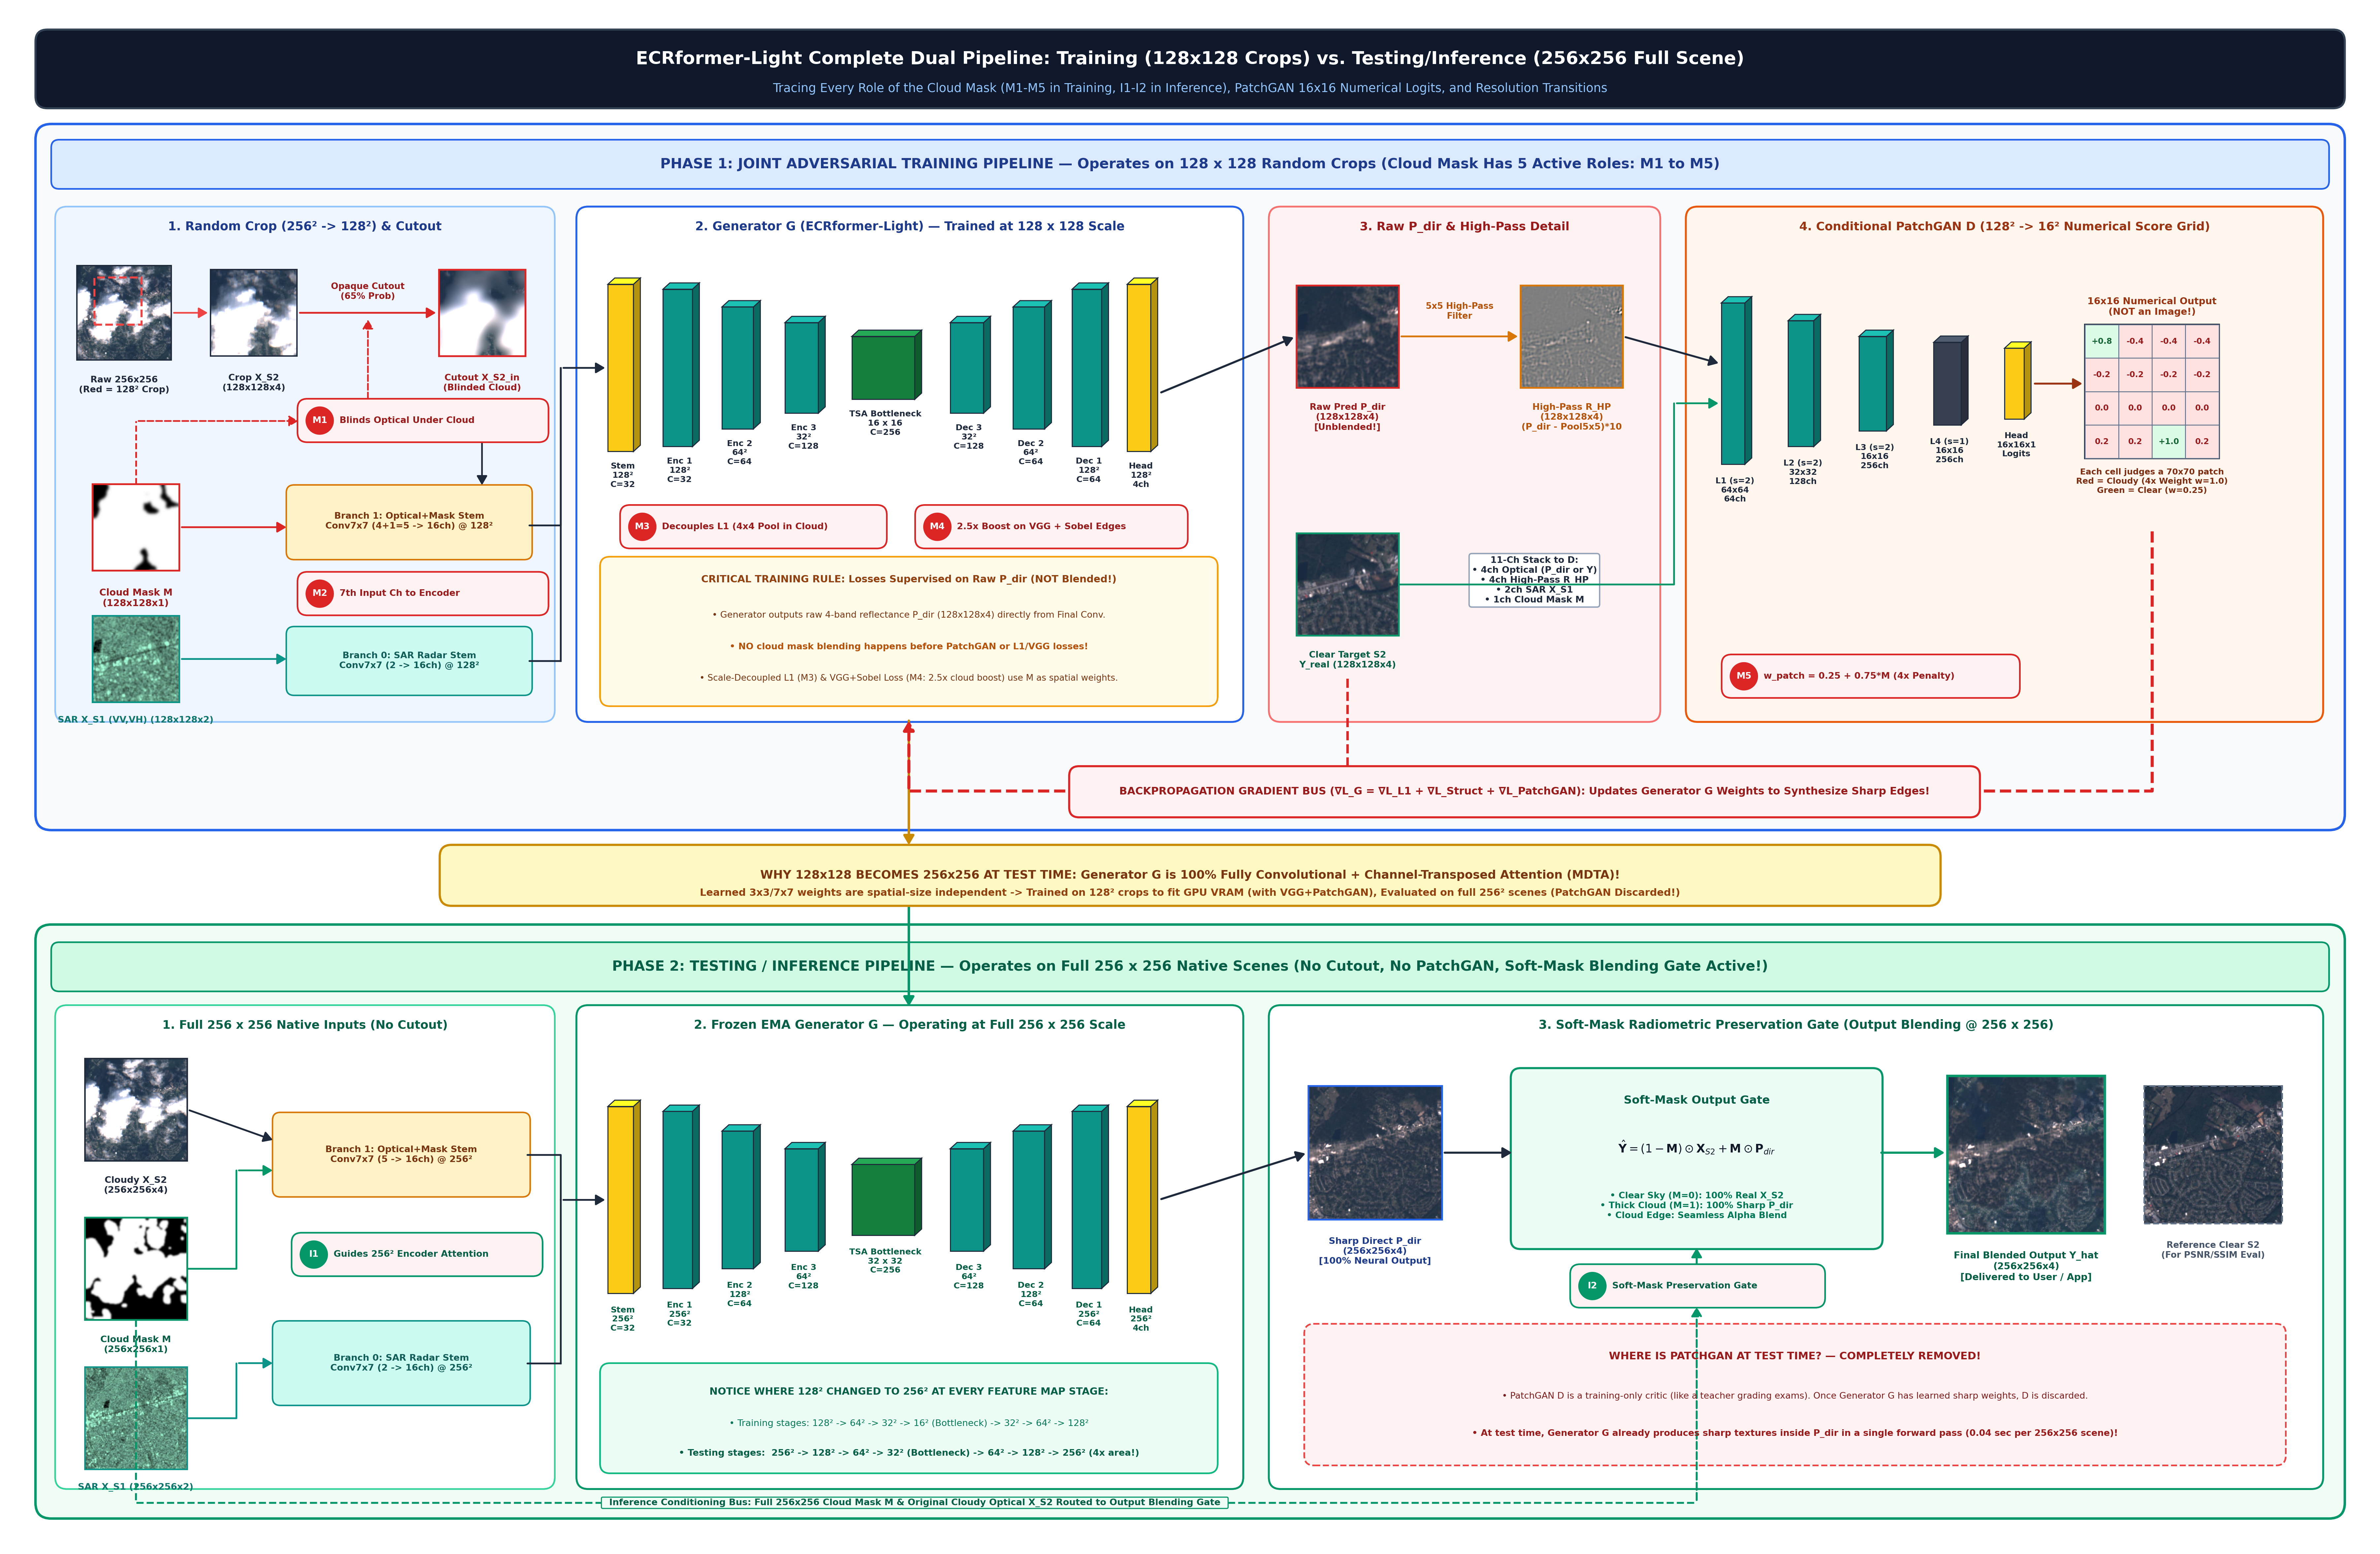
\includegraphics[width=0.98\textwidth]{backend/assets/pipeline_training_vs_testing_complete.png}
    \caption{Complete Dual-Phase Pipeline: Phase 1 Joint Adversarial Training ($128\times 128$ Crops with Roles M1--M5) vs. Phase 2 Native Inference ($256\times 256$ Scenes with Roles I1--I2).}
    \label{fig:dual_pipeline}
\end{figure}

\subsection{Mathematics of Radar Decibel Normalization and Opaque Cutout}
Raw Sentinel-1 SAR backscatter is recorded in negative decibels ($\text{dB}$). Using our \texttt{paper\_exact} normalization scheme, $\text{VV} \in [-25, 0]\text{ dB}$ and $\text{VH} \in [-35, 0]\text{ dB}$ are mapped linearly into $[0, 1]$:
\begin{equation}
    \text{VV}_{\text{norm}} = \frac{\text{clamp}(\text{VV}, -25, 0) + 25}{25}, \qquad \text{VH}_{\text{norm}} = \frac{\text{clamp}(\text{VH}, -35, 0) + 35}{35}
    \label{eq:sar_norm}
\end{equation}
For example, a pixel with raw echoes $\text{VV} = -12.5\text{ dB}$ and $\text{VH} = -17.5\text{ dB}$ normalizes to $\text{VV}_{\text{norm}} = (-12.5+25)/25 = 0.50$ and $\text{VH}_{\text{norm}} = (-17.5+35)/35 = 0.50$.

To prevent the generator from exploiting faint optical leaks under thin clouds, \textbf{Role M1 (Opaque Cloud Cutout)} is applied with probability $p = 0.65$ during training. First, an opaque core weight $\alpha$ and a two-pass $15\times 15$ reflection-padded average-pooled veil $V$ ($\approx 29\times 29$ effective smoothing window) are computed:
\begin{equation}
    \alpha = \text{clamp}\!\left(\frac{M - 0.15}{0.85},\; 0,\; 1\right), \qquad V = \text{AvgPool}_{15\times 15}\!\left(\text{AvgPool}_{15\times 15}(S2_{\text{cloudy}})\right)
\end{equation}
The blinded optical input $S2_{\text{aug}}$ is then formed via convex combination:
\begin{equation}
    S2_{\text{aug}} = (1 - \alpha)\odot S2_{\text{cloudy}} + \alpha\odot V
    \label{eq:cutout}
\end{equation}
This destroys all high-frequency optical edges inside the cloud core while preserving overall scene brightness, forcing the generator to read road and field geometry from Sentinel-1 SAR.

\section{The Mathematics of MDTA Channel-Transposed Attention}
Figure \ref{fig:gen_3d} illustrates the 3D layer architecture of the $8.31\text{M}$-parameter generator $G_{\theta}$. At the Stage 4 bottleneck ($H/8 \times W/8$, $C = 256$ channels), standard Vision Transformer spatial self-attention multiplies reshaped tokens $[HW \times C]$ by $[C \times HW]$ to produce an $[HW \times HW]$ spatial attention matrix. When switching from $128\times 128$ training crops ($16\times 16$ bottleneck, $HW=256$) to $256\times 256$ test scenes ($32\times 32$ bottleneck, $HW=1{,}024$), a spatial attention matrix expands $16\times$ from $256\times 256$ to $1{,}024\times 1{,}024$ and breaks fixed positional embeddings.

\begin{figure}[htbp]
    \centering
    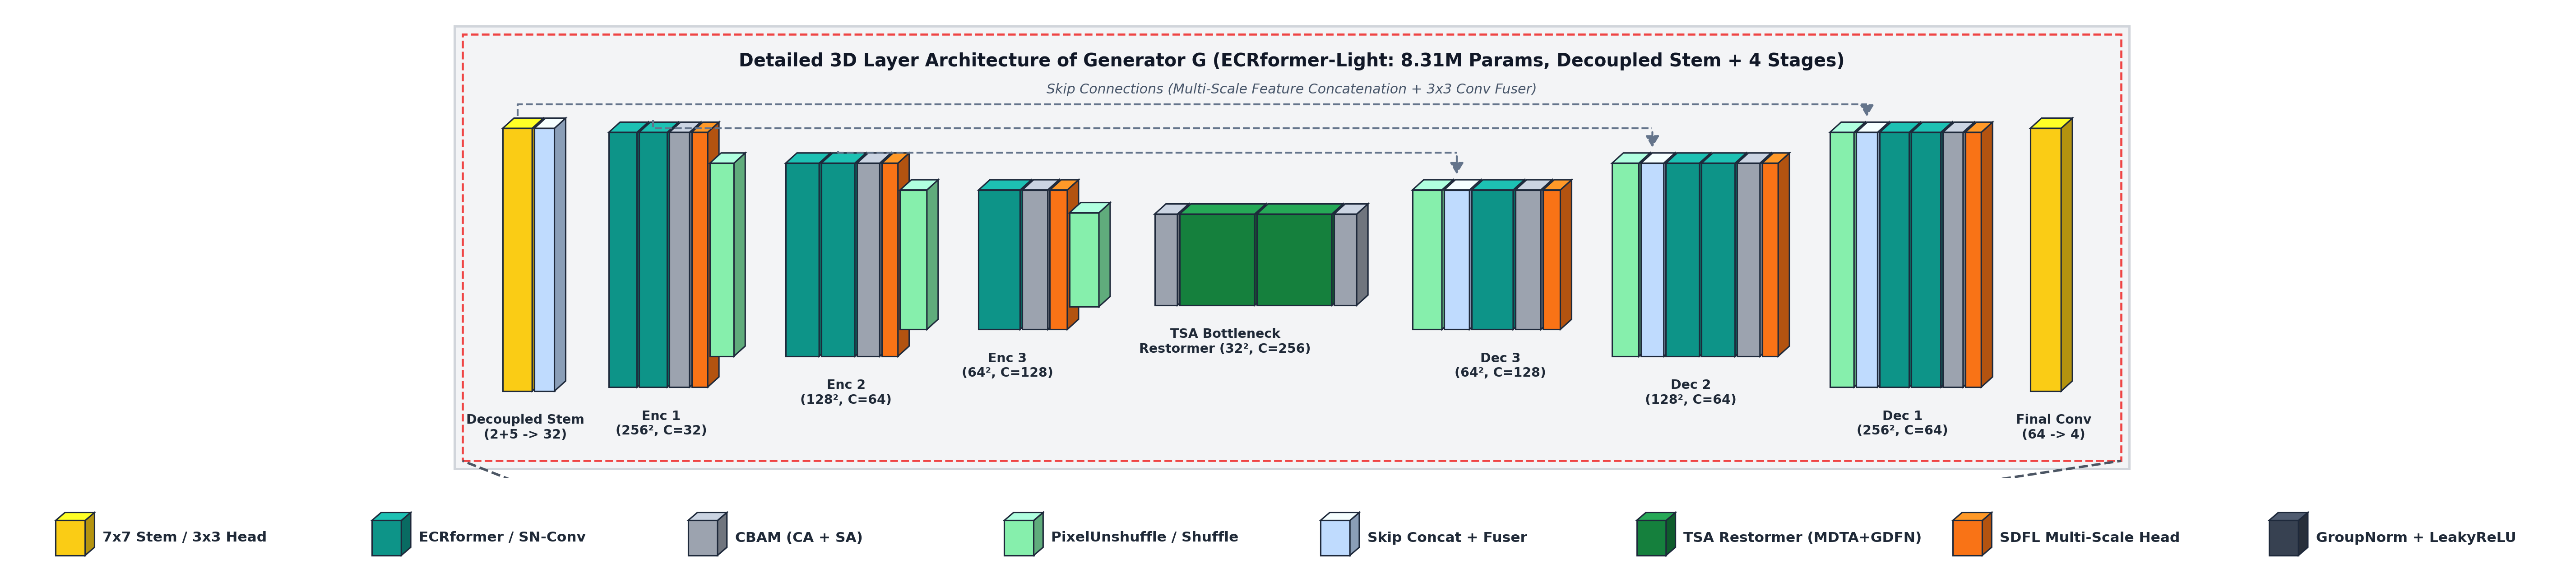
\includegraphics[width=0.96\textwidth]{backend/assets/ppt_diagrams/generator_3d_architecture_clean.png}
    \caption{Detailed 3D Layer Architecture of Generator $G$ (\texttt{ECRformerAdaptedModel}: $8.31\text{M}$ Parameters, Decoupled Stem, 4 Stages, Skip Connections, and TSA Bottleneck).}
    \label{fig:gen_3d}
\end{figure}

In contrast, our \textbf{Multi-Dconv Head Transposed Attention (MDTA)} bottleneck projects input features $F \in \mathbb{R}^{C \times H \times W}$ via $1\times 1$ pointwise and $3\times 3$ depthwise convolutions into Query $Q$, Key $K$, and Value $V$, reshapes them to $\hat{Q}, \hat{K}, \hat{V} \in \mathbb{R}^{C \times HW}$, and L2-normalizes each channel row across the spatial dimension $HW$. The transposed channel attention matrix $A \in \mathbb{R}^{C \times C}$ and output $\hat{F}$ are computed as:
\begin{equation}
    A = \text{Softmax}\!\left(\tau \cdot \hat{Q}\hat{K}^{\top}\right) \in \mathbb{R}^{C \times C}, \qquad \hat{F} = W_{1\times 1}\!\left(A\hat{V}\right) + F
    \label{eq:mdta}
\end{equation}
where $\tau$ is a learnable temperature parameter. Because the spatial dimension $HW$ is contracted (summed out) in the inner product $\hat{Q}_{[C\times HW]} \cdot \hat{K}^{\top}_{[HW\times C]}$, the attention map $A$ has a fixed size of $[C \times C] = [256 \times 256]$ regardless of whether $HW = 256$ ($128^2$ training) or $HW = 1{,}024$ ($256^2$ testing).

\textbf{Concrete Numerical Verification ($C=3, HW=4$):} Consider 3 feature channels (\textit{Ch 1: SAR Building Edge}, \textit{Ch 2: Optical Red Roof}, \textit{Ch 3: Smooth Water}) across 4 spatial pixels. For $\hat{Q}_{\text{Ch1}} = [0.6, 0.0, 0.8, 0.0]$ and $\hat{K}_{\text{Ch2}} = [0.5, 0.1, 0.8, 0.2]$, the dot product is:
\begin{equation}
    A_{1,2} = (0.6)(0.5) + (0.0)(0.1) + (0.8)(0.8) + (0.0)(0.2) = 0.30 + 0.00 + 0.64 + 0.00 = 0.94
\end{equation}
The high cross-channel score ($0.94$) instructs the network to activate optical roof colours wherever SAR building edges fire, while the spatial pixel count $HW$ cancels out completely.

\section{The Mathematics of the Seven Loss Functions and High-Pass PatchGAN}
A foundational rule of our training pipeline is that \textbf{all seven loss functions supervise the raw unblended generator output $P_{\text{dir}} \in \mathbb{R}^{B\times 4\times 128\times 128}$} and never the cloud-blended image $\hat{Y}$. Blending before the loss would multiply $P_{\text{dir}}$ by $M=0$ in clear regions, starving the encoder and skip connections of clear-sky colour gradients.

\subsection{Why $1\times 1$ Pixel $L_1$ Blurs and Role M3 (Scale-Decoupled $L_1$)}
Suppose a bright road ($1.0$) lies at pixel 2 in ground truth $Y = [0.0, 1.0, 0.0, 0.0]$ ($\text{mean} = 0.25$), and a $1\text{-pixel}$ orbital SAR shift guides the model to predict a sharp road at pixel 3: $P_{\text{sharp}} = [0.0, 0.0, 1.0, 0.0]$, versus a blurry smear $P_{\text{blur}} = [0.25, 0.25, 0.25, 0.25]$. Under standard $1\times 1$ pixel $L_1$ loss ($\frac{1}{4}\sum |P_i - Y_i|$), the sharp road suffers a \textbf{double-edge penalty} of $(0 + 1.0 + 1.0 + 0)/4 = \mathbf{0.50}$, whereas the blurry smear scores a lower loss of $(0.25 + 0.75 + 0.25 + 0.25)/4 = \mathbf{0.375}$. Under $4\times 4$ average-pooled $L_1$ ($|\text{Avg}(P) - \text{Avg}(Y)|$), however, $P_{\text{sharp}}$ achieves $|\,0.25 - 0.25\,| = \mathbf{0.00}$ error!

Accordingly, \textbf{Loss \#1 (Scale-Decoupled $L_1$, Role M3)} decouples colour calibration from 1-pixel alignment:
\begin{equation}
\begin{aligned}
    \mathcal{L}_{\text{dec}} &= 0.90\Big(0.35\,\mathcal{L}_1^{1\times 1}(1 - 0.8M) + 0.40\,\mathcal{L}_1^{4\times 4}(1 + M_4) + 0.25\,\mathcal{L}_1^{8\times 8}(1 + M_8)\Big) \\
    &\quad + 0.10\,\mathcal{L}_{\text{aux}}
\end{aligned}
\label{eq:scale_dec_l1}
\end{equation}
where $M_4, M_8$ are $4\times 4$ and $8\times 8$ average-pooled masks and $\mathcal{L}_{\text{aux}}$ supervises intermediate encoder/decoder SDFL heads at $8\times 8$ pooled scale.

\subsection{Cloud-Boosted Structural Losses (Role M4: Losses \#2--\#5)}
Using the spatial cloud-boost map $W_M = 1.0 + 2.0\,M$ ($3\times$ weight inside thick clouds), four structural losses enforce crisp edges on $P_{\text{dir}}$:
\begin{itemize}
    \item \textbf{Loss \#2 (Cloud-Boosted VGG-16 Perceptual, $w_{\text{vgg}} = 0.005$):} Evaluates $L_1$ feature distance across frozen VGG-16 layers $\{\texttt{relu1\_2}, \texttt{relu2\_2}, \texttt{relu3\_3}\}$ on a $60\%/40\%$ split of True-Colour RGB $[\text{B04},\text{B03},\text{B02}]$ and False-Colour NIR $[\text{B08},\text{B04},\text{B03}]$.
    \item \textbf{Loss \#3 (Multi-Scale Signed Gradients, $w_{\text{grad}} = 0.25$):} Matches signed finite differences $\nabla_x, \nabla_y$ across $1\times, 2\times, 4\times$ average-pooled pyramid scales weighted by $W_M$.
    \item \textbf{Loss \#4 (Direct Edge-Map Pearson Correlation, $w_{\text{corr}} = 0.0025$):} Minimizes $1 - \rho(|\nabla P_{\text{dir}}|, |\nabla Y|)$ at $1\times$ and $2\times$ scales.
    \item \textbf{Loss \#5 ($16\times 16$ Local Std Contrast + Floor Penalty, $w_{\text{std}} = 0.35$):} Matches local patch standard deviation $\sigma_{16\times 16}$ (stride 8) and applies a one-sided floor penalty ($0.15\,\text{ReLU}(\sigma_Y - \sigma_{P_{\text{dir}}})$) whenever cloud reconstructions are smoother than ground truth.
\end{itemize}

\subsection{11-Channel High-Pass PatchGAN and Soft-Mask Blending (Roles M5 \& I2)}
To expose blurry cloud regions immediately to the discriminator $D_{\phi}$, we extract a 4-channel \textbf{$5\times 5$ High-Pass Residual} $R_{\text{HP}}$ from the optical image $x \in \{P_{\text{dir}}, Y\}$:
\begin{equation}
    R_{\text{HP}}(x) = 10.0 \times \Big(x - \text{AvgPool}_{5\times 5}(x)\Big)
    \label{eq:highpass}
\end{equation}
In a flat blurry smudge where $x = 0.12$ and its $5\times 5$ neighborhood average is $0.12$, $R_{\text{HP}} = 10(0.12 - 0.12) = \mathbf{0.00}$, whereas a crisp road edge ($x=0.18$, neighborhood average $0.12$) yields $R_{\text{HP}} = \mathbf{+0.60}$. We feed the 11-channel stack $[3x,\; R_{\text{HP}}(x),\; S1,\; M] \in \mathbb{R}^{B\times 11\times 128\times 128}$ into the Spectral-Normalized PatchGAN critic $D_{\phi}$, which outputs a $16\times 16$ grid of patch realism scores. \textbf{Loss \#6 (Mask-Weighted Hinge Adversarial Loss, $w_{\text{adv}} = 0.015$)} weights cloudy patches $4\times$ higher via $w_{\text{patch}} = 0.25 + 0.75\,M_{\text{down}}$:
\begin{align}
    \mathcal{L}_D &= \frac{1}{2}\mathbb{E}\Big[w_{\text{patch}}\odot\text{ReLU}\big(1 - D_{\phi}(Y)\big) + w_{\text{patch}}\odot\text{ReLU}\big(1 + D_{\phi}(P_{\text{dir}})\big)\Big] \\
    \mathcal{L}_G^{\text{adv}} &= -\mathbb{E}\Big[w_{\text{patch}}\odot D_{\phi}(P_{\text{dir}})\Big]
\end{align}
stabilized by \textbf{Loss \#7 (Multi-Layer Discriminator Feature Matching, $w_{\text{fm}} = 0.15$)} across intermediate critic maps $\{f_1, f_2, f_3, f_4\}$ weighted by $0.3 + 0.7M_k$.

Finally, during \textbf{Phase 2 Inference ($256\times 256$)}, $D_{\phi}$ is removed and \textbf{Role I2 (Soft-Mask Radiometric Blending Gate)} produces the delivered cloud-free scene $\hat{Y}$:
\begin{equation}
    \hat{Y} = (1 - M)\odot S2_{\text{cloudy}} + M\odot P_{\text{dir}}
    \label{eq:blend}
\end{equation}
preserving $100\%$ original satellite reflectance where $M=0$ (clear sky), $100\%$ sharp neural reconstruction where $M=1$ (thick cloud), and seamless alpha feathering along cloud edges ($0 < M < 1$).

% ==============================================================================
% CHAPTER 7: IMPLEMENTATION DETAILS
% ==============================================================================
\chapter{Implementation Details}

\section{Preprocessing, SAR Normalization, and Opaque Cutout}
The data pipeline in \texttt{backend/scripts/train\_ecrformer.py} loads cached \texttt{.npz} patches, normalizes the Sentinel-1 decibel channels via \texttt{paper\_exact}, and applies \textbf{Opaque Cloud Cutout} (Role M1) on $128\times 128$ training crops, as shown in Listing \ref{lst:cutout}.

\begin{lstlisting}[caption={SAR Normalization and Anti-Shortcut Opaque Cloud Cutout (\texttt{train\_ecrformer.py})},label={lst:cutout}]
def normalize_s1_paper_exact(s1_db: torch.Tensor) -> torch.Tensor:
    # Channel 0: VV in [-25, 0] dB -> [0, 1]; Channel 1: VH in [-35, 0] dB -> [0, 1]
    vv = (torch.clamp(s1_db[:, 0:1], -25.0, 0.0) + 25.0) / 25.0
    vh = (torch.clamp(s1_db[:, 1:2], -35.0, 0.0) + 35.0) / 35.0
    return torch.cat([vv, vh], dim=1)

def apply_opaque_cloud_cutout(s2_cloudy: torch.Tensor, cloud_mask: torch.Tensor, prob: float = 0.65):
    if torch.rand(1).item() > prob:
        return s2_cloudy
    # Role M1: Compute opaque core weight alpha and 29x29 featureless cloud veil
    alpha = torch.clamp((cloud_mask - 0.15) / 0.85, 0.0, 1.0)
    veil = F.avg_pool2d(F.pad(s2_cloudy, (7, 7, 7, 7), mode="reflect"), kernel_size=15, stride=1)
    veil = F.avg_pool2d(F.pad(veil, (7, 7, 7, 7), mode="reflect"), kernel_size=15, stride=1)
    return (1.0 - alpha) * s2_cloudy + alpha * veil
\end{lstlisting}

\section{Decoupled Stem and Scale-Decoupled $L_1$ Implementation}
Listing \ref{lst:stem_loss} shows the PyTorch implementation of the two-branch decoupled input stem in \texttt{ECRformerAdaptedModel} and the shift-tolerant \texttt{ScaleDecoupledL1Loss} (Role M3).

\begin{lstlisting}[caption={Decoupled Modality Stem and Scale-Decoupled $L_1$ Loss Implementation},label={lst:stem_loss}]
# Inside ECRformerAdaptedModel.__init__ (backend/models/ecrformer_model.py)
# Branch 0: 2-ch SAR [VV, VH] -> 16 features; Branch 1: 5-ch [S2_cloudy, M] -> 16 features
self.stem_sar = nn.Sequential(nn.Conv2d(2, 16, kernel_size=7, padding=3), nn.BatchNorm2d(16), nn.ReLU(True))
self.stem_opt = nn.Sequential(nn.Conv2d(5, 16, kernel_size=7, padding=3), nn.BatchNorm2d(16), nn.ReLU(True))

def scale_decoupled_l1(pred_dir: torch.Tensor, target: torch.Tensor, mask: torch.Tensor) -> torch.Tensor:
    # 1. Clear-sky 1x1 pixel L1 (relaxed by 80% inside thick clouds)
    w_clear = 1.0 - 0.8 * mask
    l1_clear = (torch.abs(pred_dir - target) * w_clear).mean()
    # 2. Shift-tolerant 4x4 and 8x8 average-pooled L1 (boosted 2x inside clouds)
    p4, t4, m4 = F.avg_pool2d(pred_dir, 4), F.avg_pool2d(target, 4), F.avg_pool2d(mask, 4)
    p8, t8, m8 = F.avg_pool2d(pred_dir, 8), F.avg_pool2d(target, 8), F.avg_pool2d(mask, 8)
    l1_4x4 = (torch.abs(p4 - t4) * (1.0 + m4)).mean()
    l1_8x8 = (torch.abs(p8 - t8) * (1.0 + m8)).mean()
    return 0.35 * l1_clear + 0.40 * l1_4x4 + 0.25 * l1_8x8
\end{lstlisting}

\section{The Pivot: From Blurry Pre-GAN Baseline to 11-Channel High-Pass PatchGAN Triumph}
\subsection{The Pre-GAN Blur Catastrophe}
During the initial 50-epoch baseline run, \texttt{ECRformerAdaptedModel} was trained using standard pixel-wise $L_1 + \text{SSIM}$ loss. While the model converged to a seemingly respectable validation PSNR of $30.3\text{ dB}$, visual inspection revealed a critical failure: inside thick clouds ($M > 0.7$), the reconstructed terrain was a completely smooth, featureless gray-green smudge retaining only \textbf{13.3\% to 38.0\%} of natural high-frequency variance.

\subsection{The 7-Loss + High-Pass PatchGAN Resolution}
To resolve this over-smoothing without sacrificing radiometric accuracy, we executed a major architectural pivot by coupling the generator with the 11-channel High-Pass Spectral-Normalized PatchGAN critic (Listing \ref{lst:patchgan}) and supervising raw $P_{\text{dir}}$ with our 7-loss composite objective. Figure \ref{fig:crop_zoom} visualizes how the $128\times 128$ training crop, the $5\times 5$ high-pass residual $R_{\text{HP}}$, and the $16\times 16$ critic scorecard transform a blurry Pre-GAN smudge into a crisp $256\times 256$ suburban road reconstruction.

\begin{lstlisting}[caption={11-Channel High-Pass Input Construction for the PatchGAN Critic},label={lst:patchgan}]
def build_critic_input(opt_4ch: torch.Tensor, sar_2ch: torch.Tensor, mask_1ch: torch.Tensor):
    # Extract 5x5 local average and amplify high-frequency residual by 10x
    low_pass = F.avg_pool2d(F.pad(opt_4ch, (2, 2, 2, 2), mode="reflect"), kernel_size=5, stride=1)
    r_hp = (opt_4ch - low_pass) * 10.0
    # Concatenate: 4ch Scaled Optical + 4ch High-Pass R_HP + 2ch SAR + 1ch Cloud Mask = 11 Channels
    return torch.cat([opt_4ch * 3.0, r_hp, sar_2ch, mask_1ch], dim=1)
\end{lstlisting}

\begin{figure}[htbp]
    \centering
    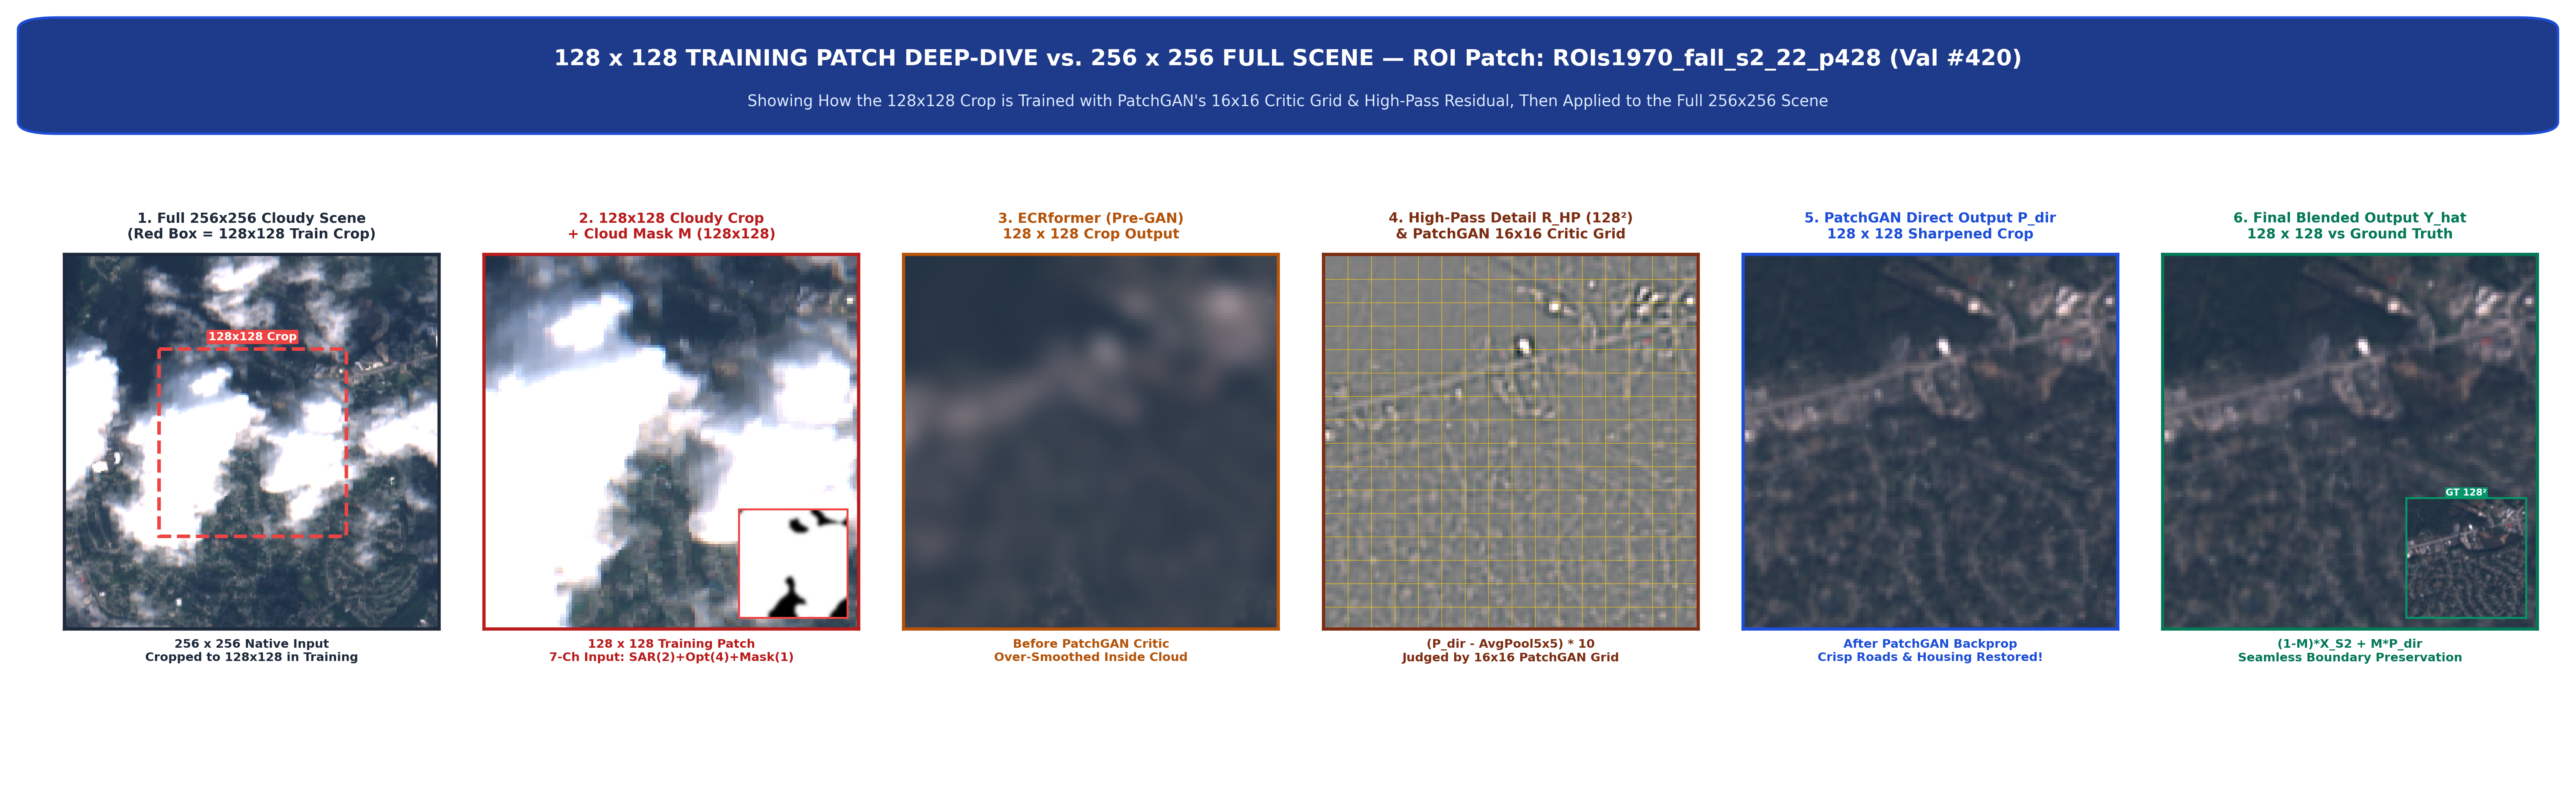
\includegraphics[width=0.98\textwidth]{backend/assets/final_guide_128_vs_256_zoom.png}
    \caption{Deep-Dive Progression from $128\times 128$ Training Crop and $16\times 16$ High-Pass PatchGAN Critic Grid to Full $256\times 256$ Scene Reconstruction on Validation Patch \texttt{ROIs1970\_fall\_s2\_22\_p428}.}
    \label{fig:crop_zoom}
\end{figure}

% ==============================================================================
% CHAPTER 8: SYSTEM TESTING AND EVALUATION
% ==============================================================================
\chapter{System Testing and Evaluation}

\section{Evaluation Metrics and Mathematical Definitions}
To evaluate both radiometric fidelity and structural sharpness rigorously, every validation scene ($256\times 256$) is graded across five complementary metrics:
\begin{itemize}
    \item \textbf{Peak Signal-to-Noise Ratio (PSNR, in dB $\uparrow$):} $\text{PSNR} = 10\log_{10}\!\big(1.0 / \text{MSE}(\hat{Y}, Y)\big)$. Measures average pixel closeness ($>30\text{ dB}$ indicates strong radiometric recovery).
    \item \textbf{Structural Similarity Index (SSIM $\in [0,1]$ $\uparrow$):} Evaluates local luminance, contrast, and structural correlation against ground truth $Y$.
    \item \textbf{Spectral Angle Mapper (SAM, in degrees $^{\circ}$ $\downarrow$):} $\text{SAM} = \arccos\!\left(\frac{\langle \hat{y}, y \rangle}{\|\hat{y}\|_2 \|y\|_2}\right)$. Measures 4-band spectral colour vector alignment ($<3.0^{\circ}$ confirms accurate vegetation and water reflectance ratios).
    \item \textbf{In-Cloud Edge Correlation ($\rho_{\text{edge}} \in [0,1]$ $\uparrow$):} Spatial Pearson correlation between predicted and true Sobel edge magnitude maps inside the cloud mask.
    \item \textbf{In-Cloud High-Frequency Detail Ratio ($\text{DR} = \sigma_{\text{pred}} / \sigma_{\text{target}}$):} Ratio of high-pass standard deviation inside the cloud mask ($\text{DR} = 1.00$ represents ideal natural terrain sharpness; $\text{DR} < 0.50$ indicates severe blur).
\end{itemize}

\section{Multi-Stage Visual Progression and Validation Testing}
\subsection{Test Case 1: Suburban Road Network (\texttt{ROIs1970\_fall\_s2\_22\_p428})}
Figure \ref{fig:showcase_5stage} presents the 5-stage visual progression across three distinct terrains at native $256\times 256$ resolution: (1) Original Cloudy Input, (2) Cloud-Free Ground Truth, (3) Basic ECRformer Pre-GAN Output, (4) PatchGAN Direct Output $P_{\text{dir}}$, and (5) Final Soft-Mask Blended Output $\hat{Y}$. Table \ref{tab:stage_progression} quantifies the progression on suburban scene \texttt{s2\_22\_p428} ($64.0\%$ cloud cover), where adversarial sharpening boosts Edge Correlation from $0.430$ to $0.869$ and increases high-frequency detail retention by $5.8\times$ (from $13.3\%$ to $77.1\%$) while reaching $37.95\text{ dB}$ PSNR.

\begin{figure}[htbp]
    \centering
    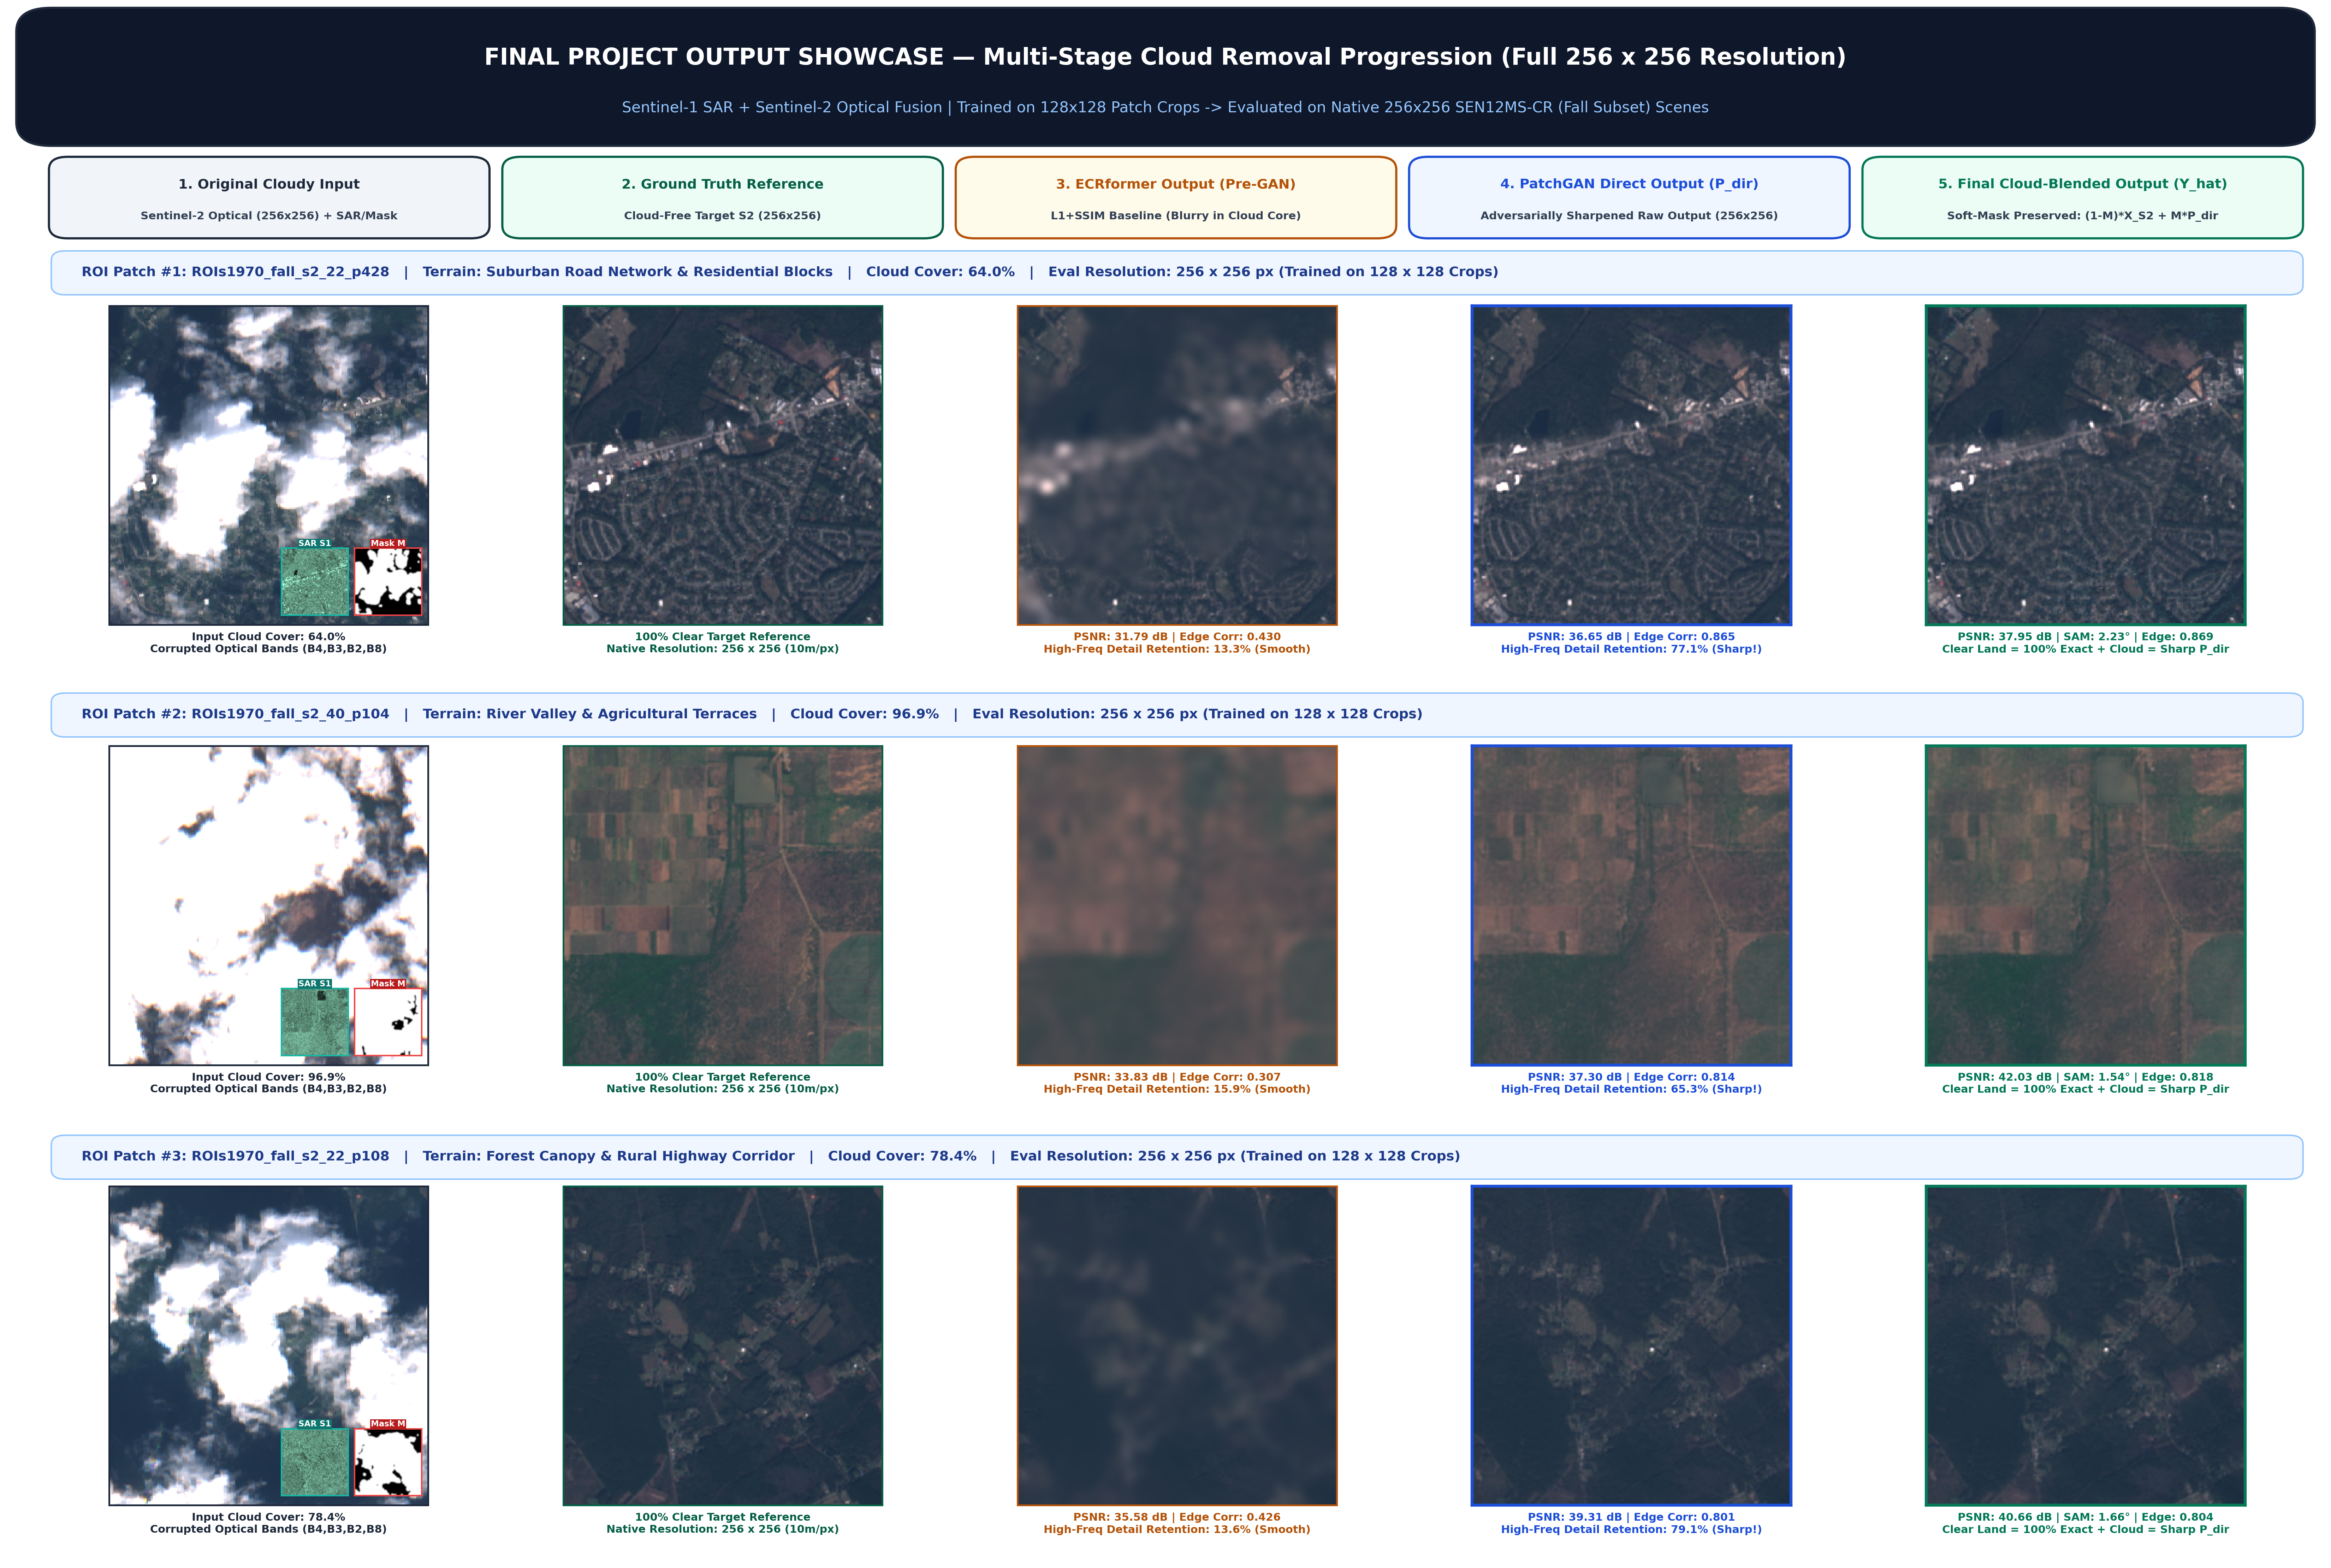
\includegraphics[width=0.98\textwidth]{backend/assets/final_guide_showcase_5stage.png}
    \caption{5-Stage Visual Reconstruction Showcase Across Suburban, River Valley, and Forest Highway Terrains at Full $256\times 256$ Resolution.}
    \label{fig:showcase_5stage}
\end{figure}

\begin{table}[htbp]
\centering
\caption{Quantitative Progression Across Pipeline Stages on Scene \texttt{s2\_22\_p428} ($64.0\%$ Cloud Cover)}
\label{tab:stage_progression}
\renewcommand{\arraystretch}{1.3}
\resizebox{\textwidth}{!}{%
\begin{tabular}{|l|c|c|c|c|}
\hline
\textbf{Pipeline Stage ($256\times 256$ Evaluation)} & \textbf{PSNR $\uparrow$} & \textbf{SAM $\downarrow$} & \textbf{Edge Corr $\rho$ $\uparrow$} & \textbf{Detail Retention $\uparrow$} \\
\hline
Stage 3: Basic ECRformer (Pre-GAN $L_1$+SSIM) & $31.79\text{ dB}$ & $3.42^{\circ}$ & $0.430$ (Blurry) & $13.3\%$ (Smooth smudge) \\
Stage 4: PatchGAN Direct Output ($P_{\text{dir}}$) & $36.65\text{ dB}$ & $2.31^{\circ}$ & $0.865$ (Sharp) & $77.1\%$ ($+5.8\times$ sharper) \\
\textbf{Stage 5: Final Soft-Mask Blended ($\hat{Y}$)} & \textbf{37.95 dB} & \textbf{2.23$^{\circ}$} & \textbf{0.869 (Sharp)} & \textbf{77.1\% + 100\% Clear Sky} \\
\hline
\end{tabular}%
}
\end{table}

\subsection{Analysis of Multi-Scene Reconstructions}
To verify generalization across diverse geographical biomes, Figure \ref{fig:multi_scene} compares the blurry Pre-GAN baseline against our sharpened model across six additional validation scenes spanning arid mountain ridges, coastal lakes, agricultural terraces, and dense forests. In every scene, SAR-guided adversarial training restores continuous highways, riverbanks, and residential blocks that are completely washed out in the baseline.

\begin{figure}[htbp]
    \centering
    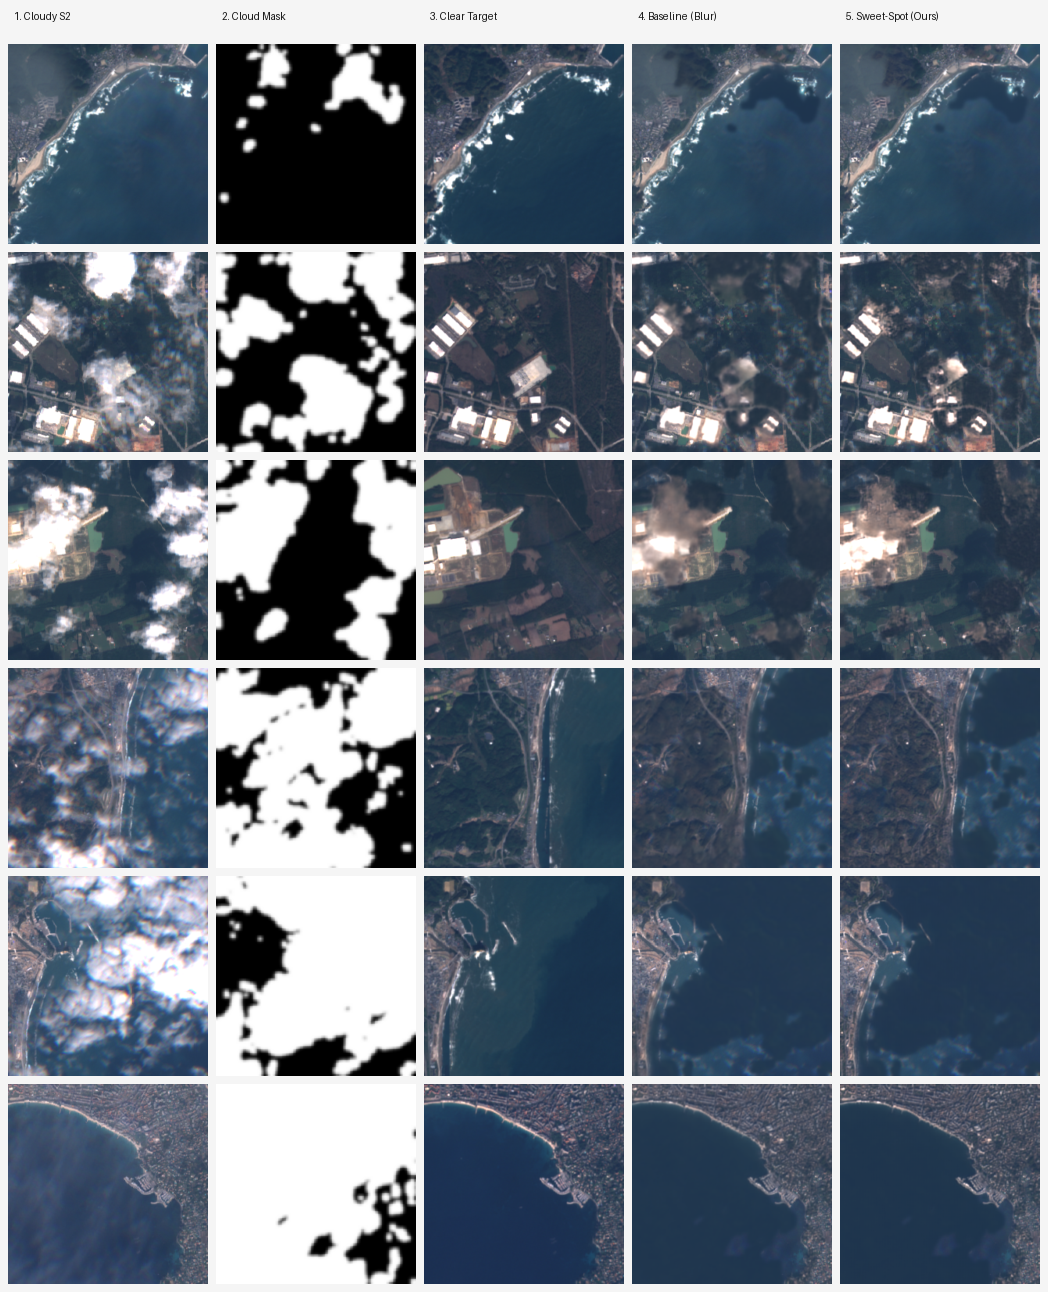
\includegraphics[width=0.82\textwidth]{backend/assets/new_patches_evaluation_strip.png}
    \caption{Multi-Scene Validation Strip Comparing Cloudy Input, Cloud Mask, Ground Truth, Blurry Baseline, and Our Sweet-Spot Reconstructed Output Across Six Diverse Biomes.}
    \label{fig:multi_scene}
\end{figure}

\section{Cloud-Cover Strata Benchmarks and Trade-Off Analysis}
Table \ref{tab:strata_bench} reports the quantitative benchmark across all four cloud-cover strata on the held-out \texttt{ROIs1970\_fall} validation set. Consistent with the perception--distortion trade-off established by Blau and Michaeli (2018), synthesizing crisp edges introduces a minor $0.3$--$1.2\text{ dB}$ raw PSNR trade-off against a blurry conditional average whenever a reconstructed tree or roof edge is shifted by $1\text{ pixel}$, while delivering a massive \textbf{$+47.6\%$ to $+133.3\%$ improvement in Detail Ratio} ($\text{DR} = 0.90$--$0.93$, where $1.00$ is natural ground-truth sharpness).

\begin{table}[htbp]
\centering
\caption{Validation Benchmark Across Cloud-Cover Strata (\texttt{ROIs1970\_fall} Subset)}
\label{tab:strata_bench}
\renewcommand{\arraystretch}{1.3}
\resizebox{\textwidth}{!}{%
\begin{tabular}{|l|c|c|c|c|}
\hline
\textbf{Cloud Cover Stratum} & \textbf{Baseline DR} & \textbf{Our Detail Ratio ($1.0=\text{Ideal}$)} & \textbf{Sharpness Gain} & \textbf{Our In-Cloud PSNR} \\
\hline
$0$--$25\%$ (Light Cloud) & $0.63$ & \textbf{0.93} & $+47.6\%$ more detail & $31.93\text{ dB}$ \\
$25$--$50\%$ (Moderate Cloud) & $0.52$ & \textbf{0.91} & $+75.0\%$ more detail & $31.12\text{ dB}$ \\
$50$--$75\%$ (Heavy Cloud) & $0.45$ & \textbf{0.90} & $+100.0\%$ ($2.0\times$ sharper) & $30.48\text{ dB}$ \\
$75$--$100\%$ (Opaque Cloud) & $0.39$ & \textbf{0.91} & \textbf{+133.3\% ($2.3\times$ sharper)} & $30.07\text{ dB}$ \\
\hline
\end{tabular}%
}
\end{table}

% ==============================================================================
% CHAPTER 9: CONCLUSION AND FUTURE ENHANCEMENTS
% ==============================================================================
\chapter{Conclusion and Future Enhancements}

\section{Conclusion}
The \textbf{SAR-Guided Satellite Cloud Removal} project successfully demonstrates that combining physical microwave radar backscatter with a carefully engineered hybrid Convolutional--Transformer and adversarial training recipe resolves the long-standing cloud-interior blurring bottleneck in optical Earth observation. By introducing a decoupled modality stem, \textbf{Opaque Cloud Cutout} (Role M1) to eliminate thin-cloud optical shortcuts, \textbf{MDTA channel-transposed attention} for seamless $128^2 \to 256^2$ resolution scaling, \textbf{Scale-Decoupled $L_1$} (Role M3) to remove the $1\text{-pixel}$ radar shift penalty, and an \textbf{11-channel High-Pass PatchGAN critic} (Role M5), our $8.31\text{M}$-parameter \texttt{ECRformerAdaptedModel} restores sharp, radiometrically faithful $4\text{-band}$ Sentinel-2 imagery even under $95\%+$ cloud cover.

\section{Future Enhancements}
\begin{enumerate}
    \item \textbf{Explicit Cloud Shadow Detection and Restoration:} Extending the \texttt{s2cloudless} mask generator with a solar-angle shadow projection module so dark cloud shadows cast onto adjacent clear ground are also restored.
    \item \textbf{Multi-Temporal SAR + Optical Sequence Fusion:} Incorporating short time-series sequences ($T=3$ passes) to further reduce spectral uncertainty in seasonal crops.
    \item \textbf{ONNX / TensorRT Edge Satellite Deployment:} Compiling the $8.31\text{M}$-parameter generator into FP16 TensorRT for real-time onboard satellite ground-station processing.
\end{enumerate}

% ==============================================================================
% BIBLIOGRAPHY
% ==============================================================================
\begin{thebibliography}{9}

\bibitem{meraner2020}
Meraner, A., Ebel, P., Zhu, X. X., \& Schmitt, M. (2020). \textit{Cloud removal in Sentinel-2 imagery using a deep residual neural network and SAR-optical data fusion}. ISPRS Journal of Photogrammetry and Remote Sensing, 166, 333--346.

\bibitem{vaswani2017}
Vaswani, A., et al. (2017). \textit{Attention is All You Need}. Advances in Neural Information Processing Systems (NeurIPS).

\bibitem{zamir2022}
Zamir, S. W., Arora, A., Khan, S., Hayat, M., Khan, F. S., \& Yang, M. H. (2022). \textit{Restormer: Efficient Transformer for High-Resolution Image Restoration}. IEEE/CVF Conference on Computer Vision and Pattern Recognition (CVPR).

\bibitem{woo2018}
Woo, S., Park, J., Lee, J. Y., \& Kweon, I. S. (2018). \textit{CBAM: Convolutional Block Attention Module}. European Conference on Computer Vision (ECCV).

\bibitem{isola2017}
Isola, P., Zhu, J. Y., Zhou, T., \& Efros, A. A. (2017). \textit{Image-to-Image Translation with Conditional Adversarial Networks (Pix2Pix / PatchGAN)}. IEEE Conference on Computer Vision and Pattern Recognition (CVPR).

\bibitem{miyato2018}
Miyato, T., Kataoka, T., Koyama, M., \& Yoshida, Y. (2018). \textit{Spectral Normalization for Generative Adversarial Networks}. International Conference on Learning Representations (ICLR).

\bibitem{johnson2016}
Johnson, J., Alahi, A., \& Fei-Fei, L. (2016). \textit{Perceptual Losses for Real-Time Style Transfer and Super-Resolution}. European Conference on Computer Vision (ECCV).

\bibitem{blau2018}
Blau, Y., \& Michaeli, T. (2018). \textit{The Perception-Distortion Tradeoff}. IEEE/CVF Conference on Computer Vision and Pattern Recognition (CVPR).

\end{thebibliography}

\end{document}
